 

\documentclass[format=acmsmall, review=false, screen=true]{acmart}

\usepackage[utf8]{inputenc}
\usepackage[english]{babel}

% Metadata Information
\acmJournal{TODAES}
%\acmVolume{9}
%\acmNumber{4}
\acmArticle{0}
\acmYear{2018}
\acmMonth{0}
\copyrightyear{2018}
%\acmArticleSeq{9}

% Copyright
%\setcopyright{acmcopyright}
%\setcopyright{acmlicensed}
%\setcopyright{rightsretained}
%\setcopyright{usgov}
%\setcopyright{usgovmixed}
%\setcopyright{cagov}
%\setcopyright{cagovmixed}

%--------- DOI ---------------------
%\acmDOI{0000001.0000001}


\usepackage{graphicx}
\usepackage{subfigure}
\usepackage{amsmath, amsthm, amssymb}
\usepackage{multirow}
%LaTeX package conflicts with several others over the use of the algorithm identifier.  
%A common indicator is something like this message: Too many }'s.l.1616     }
%To resolve the issues, simply put the following just before the inclusion of the algorithm2
\makeatletter
\newif\if@restonecol
\makeatother
\let\algorithm\relax
\let\endalgorithm\relax
\usepackage[linesnumbered,boxed,ruled]{algorithm2e}
\SetAlFnt{\small}
\SetAlCapFnt{\small}
\SetAlCapNameFnt{\small}
\SetAlCapHSkip{0pt}
\IncMargin{-\parindent}



\usepackage{csquotes}
\usepackage{indentfirst}
\usepackage{enumitem}
%\usepackage[style=acm,backend=bibtex8,maxnames=3,minnames=1,sorting=none]{biblatex}
%\usepackage{natbib}
%\bibliographystyle{unsrtnat}
\usepackage[version=4]{mhchem}
\usepackage[bottom]{footmisc}
\usepackage[normalem]{ulem}


\usepackage{afterpage}
\usepackage{comment}
% graphics path
\graphicspath{{images/}}
% figure name bold
\renewcommand{\figurename}{\textbf{Figure}}
% table name bold
\renewcommand{\tablename}{\textbf{Table}}
% footnote mark
\renewcommand{\thefootnote}{\fnsymbol{footnote}}
% add bib resource
%\addbibresource{maui.bib} 
% class format

\newtheorem{class}{Class}
%bibtex font size
\renewcommand*{\bibfont}{\footnotesize}

% correct bad hyphenation here
\hyphenation{optical networks semiconductor}

\pagenumbering{gobble}
%\usepackage{caption}
%\usepackage[font=small,labelfont=bf]{caption}


\received{0 2018}
%\received[revised]{March 2009}
%\received[accepted]{June 2009}






\begin{document}

\title[Making Aging Useful by Recycling Aging-Induced Clock Skew]{\fontsize{14}{10}\selectfont Making Aging Useful by Recycling Aging-Induced Clock Skew}

\settopmatter{printacmref=false}

\author{Tien-Hung Tseng}
\affiliation{%
  \institution{National Chiao Tung University}
  \city{Hsinchu}
  \country{Taiwan}}
\email{eric830303.cs05g@g2.nctu.edu.tw}


\author{Kai-Chiang Wu}
\affiliation{%
  \institution{National Chiao Tung University}
  \streetaddress{30 Shuangqing Rd}
  \city{Hsinchu}
  \country{Taiwan}
}
\email{kcw@cs.nctu.edu.tw}

\renewcommand{\thefootnote}{\fnsymbol{footnote}}
\begin{abstract}
Device aging, which causes significant loss on circuit performance and lifetime, has been a primary factor in reliability degradation of nanoscale designs. In this paper, we propose to take advantage of aging-induced clock skews (i.e., make them useful for aging tolerance) by manipulating and recycling these time-varying skews to compensate for the performance degradation of logic networks. The goal is to assign achievable/reasonable aging-induced clock skews in a circuit, such that its effective performance degradation due to aging can be tolerated, that is, the lifespan can be maximized.  On average, 24.95\% aging tolerance can be achieved with insignificant design overhead. Moreover, we employ $V_{th}$ assignment on clock buffers to further tolerate the aging-induced degradation of logic networks. When $V_{th}$ assignment is applied on top of aforementioned aging manipulation, the average aging tolerance can be enhanced to 37.61\%.
\end{abstract}


\begin{CCSXML}
<ccs2012>
<concept>
<concept_id>10010583.10010750</concept_id>
<concept_desc>Hardware~Robustness</concept_desc>
<concept_significance>500</concept_significance>
</concept>
<concept>
<concept_id>10010583.10010750.10010762</concept_id>
<concept_desc>Hardware~Hardware reliability</concept_desc>
<concept_significance>500</concept_significance>
</concept>
<concept>
<concept_id>10010583.10010750.10010762.10010763</concept_id>
<concept_desc>Hardware~Aging of circuits and systems</concept_desc>
<concept_significance>500</concept_significance>
</concept>
</ccs2012>
\end{CCSXML}

\ccsdesc[500]{Hardware~Robustness}
\ccsdesc[500]{Hardware~Hardware reliability}
\ccsdesc[500]{Hardware~Aging of circuits and systems}
\keywords{Clock network, Aging, Degradation, Reliability}





\maketitle

%\input abstract
\section{INTRODUCTION}
%1
The design and manufacturing of semiconductor devices have recently experienced dramatic innovations, at the cost of downgrading reliability of nanoscale integrated circuits (ICs) and system-on-chips (SOCs). The 2013 ITRS~\cite{itrs2013} projects that the long-term reliability of sub-100nm technology nodes can reach a noteworthy order of $10^3$ FITs (failures in $10^9$ hours). Soft errors, thermal and aging effects are some of the major challenges driving reliability-aware IC/SOC design techniques. With the continuous scaling of transistor dimensions, device aging, which causes temporal performance degradation and potential wear-out failure, is becoming increasingly dominant for lifetime reliability concerns because of limited timing margins~\cite{mcpherson2006reliability}. Therefore, the need of a verification and optimization flow considering aging effects emerges as a key factor in guaranteeing reliable and sustainable operation over a required lifespan.
%2
\textit{Bias temperature instability} (BTI) is known for prevailing over other device aging phenomena, in terms of dependence on the scaling of nanometer technologies. BTI~\cite{schroder2003negative} is a MOSFET aging phenomenon that occurs when transistors are stressed under bias (positive or negative, i.e., $V_{gs} = \pm V_{dd}$) at elevated temperature. As a result of the dissociation of Si-H bonds along the \ce{{Si-SiO}_2} interface, BTI-induced MOSFET aging manifests itself as an increase in the threshold voltage ($V_{th}$) and decrease in the drive current ($I_{ds}$)~\cite{stathis2006negative}, which in turn lengthen the propagation delays of logic gates/paths. Experiments on MOSFET aging~\cite{chakravarthi2004comprehensive} indicate that BTI effects grow exponentially with higher operating temperature and thinner gate oxide. If the thickness of gate oxide shrinks down to 4nm, the circuit performance can be degraded by as much as 15\% after 10 years of stress and lifetime will be dominated by BTI~\cite{kimizuka1999impact}. In contrast, when the stress condition is relaxed ($V_{gs}$ = 0), the aging mechanism can be recovered partially~\cite{kumar2006analytical} and the threshold voltage decreases toward the nominal value by more than 75\% if the recovery phase lasts sufficiently long~\cite{wang2010impact}.
%3
In addition to the aging effect on the logic gates/paths of a circuit, the impact of aging on the clock network should not be ignored. Considering both \enquote{the aging of logic networks} and \enquote{the aging of clock networks} is essential since unbalanced aging of clock networks can greatly affect circuit performance by inducing clock skews, as a result of non-uniform increases in clock latency from the clock source to different terminals. Prior work on addressing such clock skews due to aging (i.e., aging-induced clock skews) mainly attempts to balance the aging effects on various clock sub-networks, such that aging-induced clock skews can be minimized~\cite{chen2013novel, huang2013low, chakraborty2013skew}. However, suppressing aging-induced clock skews may be difficult and costly, especially for clock-gated designs where the rate of aging varies from one clock sub-network to another~\cite{lai2014bti}.

%4
Then think about the following question: if one has to work hard on (and incur significant overhead for) minimizing aging-induced clock skews but it turns out that there still exist stubborn non-zero skews, why don't we try to take advantage of them? We do; we propose to intentionally make aging-induced clock skews useful for aging tolerance. More specifically, we compensate for the performance degradation (due to aging) of logic networks by exploring \enquote{useful} clock skews, based on the concept of time borrowing. There are two key idea in our framework: (1) The first idea is to manipulate the rates of aging on different clock branches. Note that the rate of aging depends on the stress time, defined as the amount of time during which a PMOS/NMOS transistor is stressed under negative/positive bias. For clock drivers (comprising pairs of inverters), their stress times are proportional to the duty cycle of the clock signal. Therefore, our aging manipulation on clock branches is implemented by changing the duty cycle of a clock waveform delivered to each of the clock branches. (2) The second idea is based on V\textsubscript{th} assignment. That is, the threshold voltages of  certain clock buffers are replaced with higher value, such that the delay of the clock buffers are lengthened. The two idea are utilized together to implement the concept of timing borrowing in the designs. The proposed framework succeeds in mitigating effective aging-induced performance degradation, with little design penalty.
%MAUI DATE 2018
%4
\begin{comment}
Then think about the following question: if one has to work hard on (and incur significant overhead for) minimizing aging-induced clock skews but it turns out that there still exist stubborn non-zero skews, why don't we try to take advantage of them? We do; we propose to intentionally make aging-induced clock skews useful for aging tolerance. More specifically, we compensate for the performance degradation (due to aging) of logic networks by exploring \enquote{useful} aging-induced clock skews, based on the concept of time borrowing. Note that the rate of aging depends on the stress time, defined as the amount of time during which a PMOS/NMOS transistor is stressed under negative/positive bias. For clock drivers (comprising pairs of inverters), their stress times are proportional to the duty cycle of the clock signal. The key idea of our framework is to manipulate the rates of aging on different clock branches, by changing the duty cycle of a clock waveform delivered to each of the clock branches. The proposed framework succeeds in mitigating effective aging-induced performance degradation with little design penalty.
\end{comment}
\section{RELATED WORK AND PAPER CONTRIBUTION}
\label{sec:related}
\subsection{Previous Work on Aging-Aware Optimization}
\label{subsec:rw}
To deal with aging phenomena, traditional design methods adopt guard-banding by adding extra timing margins, which in practice imply over-design and may be expensive. To avoid overly conservatism, the mitigation of aging-induced performance degradation can be formulated as a timing-constrained area minimization problem with consideration of aging effects. Existing aging-aware techniques basically follow this formulation. A novel technology mapper considering signal probabilities for NBTI was developed in~\cite{kumar2007nbti}. On average, 10\% area recovery and 12\% power saving are accomplished, as compared to the most pessimistic case assuming static NBTI on all PMOS transistors in the design. The authors of~\cite{paul2006temporal} proposed a gate sizing algorithm based on Lagrangian relaxation. An average of 8.7\% area penalty is required to ensure reliable operation for 10 years. Other methods related to gate or transistor sizing can be found in~\cite{kang2007efficient},~\cite{yang2007combating}.

Aforementioned methods focus on mitigating the aging of logic networks only. There are some work~\cite{huang2013low, chakraborty2013skew,chen2013novel} addressing the aging problem of clock networks. Methodology of~\cite{chen2013novel} is also based on $V_{th}$ assignment for clock buffers. Authors of ~\cite{huang2013low} and ~\cite{chakraborty2013skew} explore the use of alternative clock gating cells for clock-gated designs. On the other hand, two new clock gating cells were presented in~\cite{lai2014bti} to balance the delay degradation of clock signal propagation, which reduces aging-induced clock skews between ungated and gated clock branches. The above work ~\cite{huang2013low, chakraborty2013skew,chen2013novel,lai2014bti} aim to minimize aging-induced clock skew instead of making it useful (i.e., assign specific clock skews in the designs to mitigate the aging-induced performance degradation).
%Aforementioned methods focus on mitigating the aging of logic networks only. To address the aging problem of clock networks,~\cite{chen2013novel, huang2013low, chakraborty2013skew} aim to minimize aging-induced clock skews by balancing the aging effects on various clock sub-networks. While~\cite{chen2013novel} is based on $V_{th}$ assignment for clock buffers,~\cite{huang2013low},~\cite{chakraborty2013skew} explore the use of alternative clock gating cells for clock-gated designs. On the other hand, two new clock gating cells were presented in~\cite{lai2014bti} to balance the delay degradation of clock signal propagation, which reduces aging-induced clock skews between ungated and gated clock branches.

\subsection{Paper Contribution}
\label{subsec:pc}
In this paper, we propose an optimization framework for aging tolerance. Our proposed framework reassigns the threshold voltage of clock buffers and manipulates the rates of aging on different clock branches, which is achieved by changing the duty cycle of a clock waveform delivered to each of the clock branches. The contributions and advantages of this work are threefold:
%In this paper, we propose an optimization framework, MAUI (Making Aging Useful, Intentionally), for aging tolerance. Our proposed framework manipulates the rates of aging on different clock branches, by changing the duty cycle of a clock waveform delivered to each of the clock branches. The contributions and advantages of this work are threefold:




\begin{itemize}
\item \textbf{\textit{Exploration of aging-induced clock skews for aging tolerance:}} Existing work on addressing aging-induced clock skews mainly attempts to minimize the skews. This paper presents the first work on \textit{exploring \enquote{useful} clock skews (i.e., making them useful)} for aging tolerance\footnote[1]{We do not minimize \enquote{absolute} performance degradation by directly mitigating the aging of logic networks; instead; we minimize \enquote{effective} performance degradation by $V_{th}$ assignment and manipulation of aging rates on clock networks. Furthermore, the aging of logic network is tolerated based on timing borrowing, as a result of newly-designated clock skews in designs, which is achieved by $V_{th}$ assignment and aging manipulation on clock networks. Of course, one can mitigate the logic's aging itself by using existing techniques~\cite{kumar2007nbti, paul2006temporal, kang2007efficient, yang2007combating} before applying the proposed framework. This is however beyond the scope of this work and thus not particularly addressed in this paper.}.
\item  \textbf{\textit{Problem formulation based on Boolean satisfiability and optimal solutions:}} The proposed formulation of making clock skew useful is transformed into a Boolean satisfiability (SAT) problem, and its optimal solution can be efficiently found by a SAT solver such as MiniSat.
\item \textbf{\textit{Low design overhead and little design modification:}} Restrained by the synthesized clock tree whose topology and structure are basically determined, our post-CTS (clock tree synthesis) framework does not involve aggressive modification and thus does not incur significant design overhead.
\end{itemize}



%\begin{itemize}
%\item \textbf{\textit{Exploration of aging-induced clock skews for aging tolerance:}} Existing work on addressing aging-induced clock skews mainly attempts to minimize the skews. This paper presents the first work on \textit{exploring \enquote{useful} aging-induced clock skews (i.e., making them useful)} for aging tolerance\footnote[1]{We do not minimize \enquote{absolute} performance degradation by mitigating the aging of logic networks; instead; we minimize \enquote{effective} performance degradation by manipulating the aging of clock networks to \enquote{tolerate} expected logic's aging based on time borrowing, as a result of aging-induced clock skews. Of course, one can mitigate the logic's aging itself by using existing techniques~\cite{kumar2007nbti, paul2006temporal, kang2007efficient, yang2007combating} before applying the proposed framework. This is however beyond the scope of this work and thus not particularly addressed in this paper.}.
%\item  \textbf{\textit{Problem formulation based on Boolean satisfiability and optimal solutions:}} The proposed formulation of making aging useful is transformed into a Boolean satisfiability (SAT) problem, and its optimal solution can be efficiently found by a SAT solver such as MiniSat.
%\item \textbf{\textit{Low design overhead and little design modification:}} Restrained by the synthesized clock tree whose topology and structure are basically determined, our post-CTS (clock tree synthesis) framework does not involve aggressive modification and thus does not incur significant design overhead.
%\end{itemize}
\section{MOTIVATING EXAMPLE}
\label{sec:motivate}
\begin{figure*}[!ht]
    \centering
    \subfigure[Example]{
    	\label{fig:sub:example}
        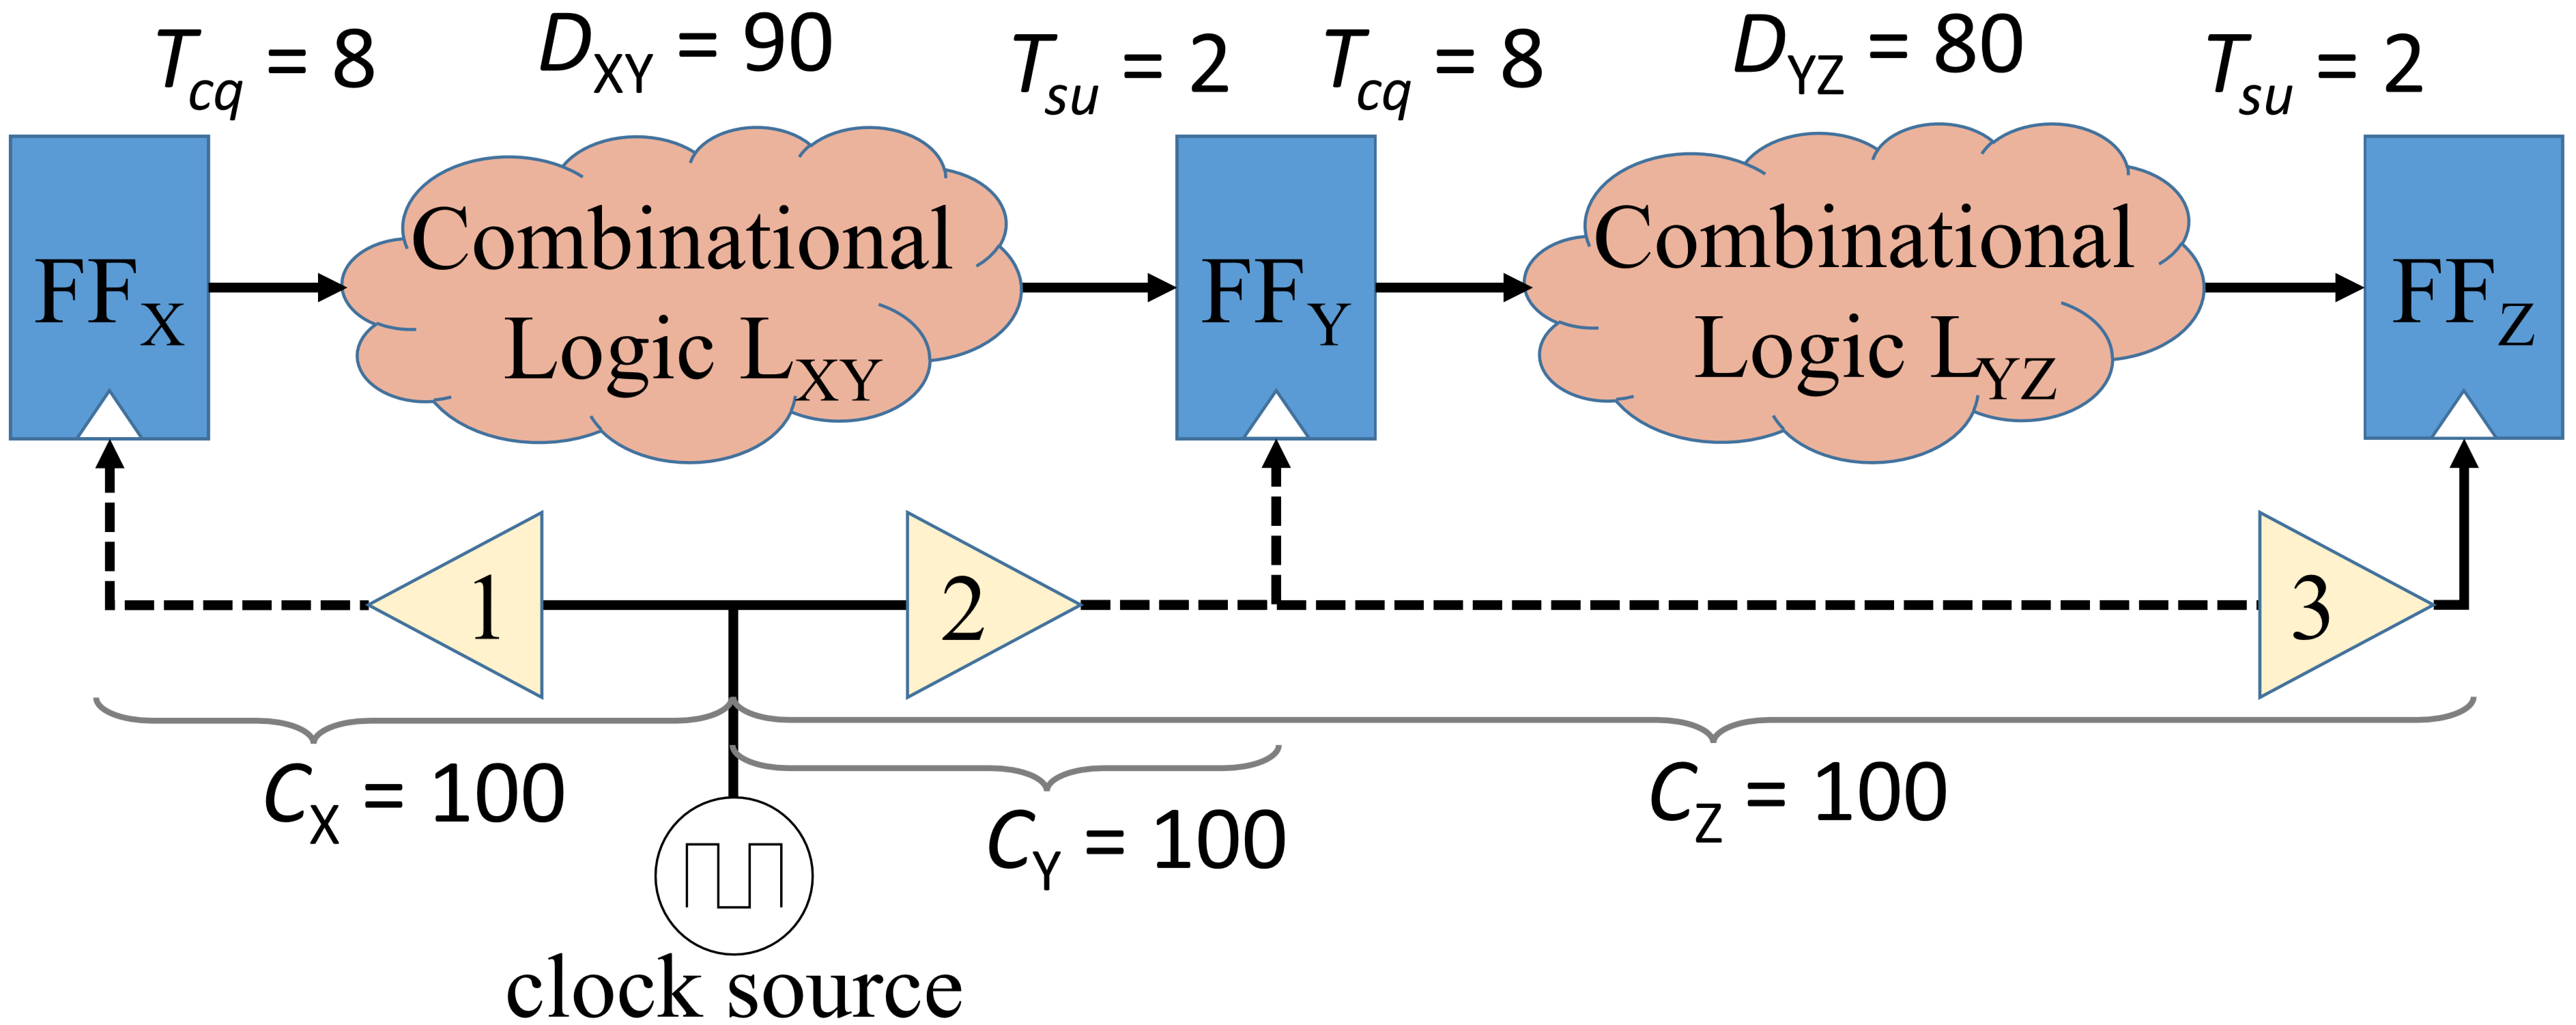
\includegraphics[width=0.9\columnwidth]{Motivating_example.png}
    }
    \hspace{1.6cm}
    \subfigure[Notations]{
    	\label{fig:sub:notations}
        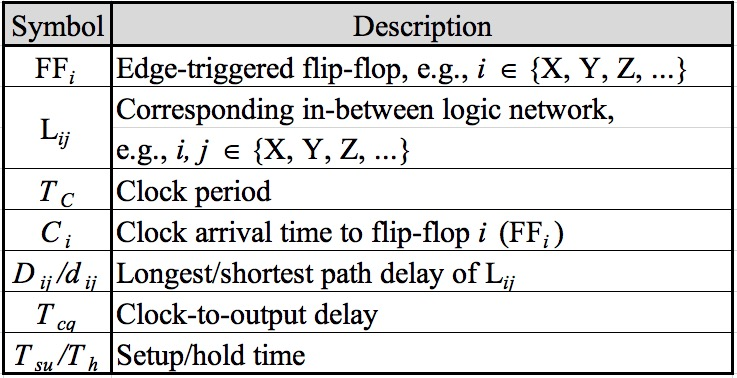
\includegraphics[width=0.8\columnwidth]{Notations.png}
    }
    \caption{Illustrative example and notations for the proposed framework based on DCC deployment/insertion}
    \label{fig:en}
\end{figure*}


This section introduces two illustrative examples which motivates our idea of making clock skew useful, based on the two methodologies: ($i$) Manipulate the aging behaviors of clock paths, introduced in Section~\ref{sec:mot:exp1}. ($ii$) Reassign the $V_{th}$ of clock buffers, introduced in Section~\ref{sec:mot:exp2}. %The section is organized as follows: Section~\ref{sec:mot:exp1} details how aging tolerance can be achieved based on ($i$). Then, Section~\ref{sec:mot:exp2} details how aging tolerance can be further improved by ($ii$). Finally, Section~\ref{subsec:apm} and Section~\ref{sec:mot:$V_{th}^{h}$} introduce the timing model of aging prediction and high-$V_{th}$ clock buffers.

\subsection{Aging Manipulation of Clock Paths}
\label{sec:mot:exp1}
Consider the circuit in Figure~\ref{fig:sub:example} where \ce{FF_X}, \ce{FF_Y} and \ce{FF_Z} are three edge-triggered flip-flops, and \ce{L_{XY}} and \ce{L_{YZ}} are the corresponding in-between logic networks. Other notations to be used later are listed in Figure~\ref{fig:sub:notations}.

For each pair of flip-flops (e.g., \ce{FF_i} and \ce{FF_j}) between which there exists at least one logic path from \ce{FF_i} to \ce{FF_j}, the following setup-time (Equation (\ref{eq:tsu})) and hold-time (Equation (\ref{eq:th})) constraints need to be satisfied:
\begin{equation}
	\mbox{\fontsize{9}{9.6} $C_i+T_{cq}+D_{ij}+T_{su}<C_j+T_c$}
	\label{eq:tsu}
\end{equation}
\begin{equation}
	\mbox{\fontsize{9}{9.6} $C_i+T_{cq}+d_{ij}<C_j+T_h$}
	\label{eq:th}
\end{equation}

Assume that, at year 10, $D_{ij}$ is degraded by 15\%, and both $T_{cq}$ and $T_{su}$ increase by 20\%. By using the predictive model presented in~\cite{wang2010impact},~\cite{wang2007efficient}, we can accurately derive the aging of $C_i$ and $C_j$ due to the regularity and predictability of a typical clock waveform of 50\% duty cycle. In the process technology used (TSMC 45nm GP standard cell series), $C_i$ and $C_j$ are degraded by 13\% under 10-year BTI, i.e., $C_i$ and $C_j$ become 1.13X larger.

To be aging-aware for the example circuit in Figure~\ref{fig:sub:example}, we have to consider aforementioned aging factors in the setup-time constraints on \ce{L_{XY}} and \ce{L_{YZ}}:
\begin{equation}
\mbox{\fontsize{9}{9.6}\selectfont \ce{L_{XY}}:\quad$\textbf{1.13}C_X+1.2T_{cq}+1.15D_{XY}+1.2T_{su}<\textbf{1.13}C_Y+T_c$} 
\label{eq:lxy}
\end{equation}
\begin{equation}
\mbox{\fontsize{9}{9.6}\selectfont \ce{L_{YZ}}:$\quad\textbf{1.13}C_Y+1.2T_{cq}+1.15D_{YZ}+1.2T_{su}<\textbf{1.13}C_Z+T_c$} 
\label{eq:lyz}
\end{equation}
where $C_X$ = $C_Y$ = $C_Z$ = 100, $T_{cq}$ = 8, $T_{su}$ = 2, $D_{XY}$ = 90 and $D_{YZ}$ = 80, as shown in Figure~\ref{fig:sub:example}.
\begin{flushleft}
By re-arranging Equations (\ref{eq:lxy}) and (\ref{eq:lyz}):
\begin{flalign*}
\hspace{1.2em}\ce{L_{XY}}: T_c &> 115.5 &\\
\hspace{1.2em}\ce{L_{YZ}}: T_c &> 104
\end{flalign*}
\end {flushleft}
Therefore, the clock period needs to be larger than 115.5 (dominated by \ce{L_{XY}}) to ensure no setup-time violation over a required lifespan of 10 years. For brevity, we omit the discussion on hold-time constraints, which in our work are actually formulated to ensure no existence of racing due to short paths.

To minimize required $T_c$ under aging, we use \textit{duty-cycle converter} (DCC) to manipulate the aging rates of clock branches. We insert one 20\% DCC at the input of buffer 1, and another 80\% DCC at the input of buffer 2. The 20\% (80\%) DCC can decrease (increase) the stress times of downstream clock buffers by converting the clock duty cycle to 20\% (80\%), from a typical duty cycle of 50\%. Therefore, 20\% DCC can mitigate/decelerate the aging of $C_X$ and 80\% DCC can aggravate/accelerate the aging of $C_Y$. In the case of no DCC, $C_X$ and $C_Y$ are degraded by 13\% under 10-year BTI in TSMC 45nm GP standard cell series, while 20\% and 80\% DCCs will degrade $C_X$ and $C_Y$ by 9\% and 16\%, respectively, assuming that the clock paths from the clock source to \ce{FF_X} and \ce{FF_Y} are disjoint.

Consider the new aging factors (due to effects of various clock duty cycles) in the setup-time constraints on \ce{L_{XY}} and \ce{L_{YZ}}:
\begin{equation}
\mbox{\fontsize{9}{9.6}\selectfont \ce{L_{XY}}:\quad$\textbf{1.09}C_X+1.2T_{cq}+1.15D_{XY}+1.2T_{su}<\textbf{1.16}C_Y+T_c$} 
\label{eq:lxy2}
\end{equation}
\begin{equation}
\centering
\mbox{\fontsize{9}{9.6}\selectfont \ce{L_{YZ}}:\quad$\textbf{1.16}C_Y+1.2T_{cq}+1.15D_{YZ}+1.2T_{su}<\textbf{1.16}C_Z+T_c$} 
\label{eq:lyz2}
\end{equation}
By re-arranging Equations (\ref{eq:lxy2}) and (\ref{eq:lyz2}):
\begin{flalign*}
\hspace{1.2em}\ce{L_{XY}}: T_c &> 108.5 &\\
\hspace{1.2em}\ce{L_{YZ}}: T_c &> 104
\end{flalign*}
As it can be seen, we can reduce the required $T_c$ from 115.5 to 108.5 (dominated by \ce{L_{XY}} still), by adding two DCCs in the existing synthesized clock tree to create aging-induced clock skews. The skew for \ce{L_{XY}} (between \ce{FF_X} and \ce{FF_Y}), quantified as 1.16$C_Y$ minus 1.09$C_X$, is useful/beneficial and accounts for the reduction of required $T_c$. A certain level of aging tolerance is thus achieved because aging-induced performance degradation of $D_{XY}$ (plus $T_{cq}$ and $T_{su}$ actually) can be tolerated, by exploring such useful aging-induced clock skews.

\subsection{High-$V_{th}$ Assignment of Clock Buffers}
\label{sec:mot:exp2}
In the example, the two approaches, High-$V_{th}$ ($V_{th}^{h}$) assignment and aging manipulation, are both applied to further optimize/reduce required $T_c$. 

Consider the circuit in Figure~\ref{fig:sub:example} again, we identically insert/deploy 20\% DCC and 80\% DCC at the inputs of buffers 1 and 2, respectively. Moreover, buffer 2 is selected as a \textit{High-$V_{th}$/$V_{th}^{h}$ buffer leader}\footnote{\textit{$V_{th}^{h}$ buffer leader} denotes that, the $V_{th}$ of downstream (toward terminals/flip-flops) clock buffers are reassigned to a specific high counterpart.}. Therefore, for the clock buffers, which are located in the intervals from buffer 2 to \ce{FF_x} and  to \ce{FF_y}, their $V_{th}$ are assigned to $V_{th}^{h}$. To include the timing information of $V_{th}^{h}$ buffers in the setup-time constraint, we assume that, the fresh/intrinsic delay of $V_{th}^{h}$ buffer is 1.2X longer than that of nominal buffer, and aging rates of $V_{th}^{h}$ buffer, with the duty cycle of 20\%, 40\%, 50\% and 80\%, are 0.5\%, 4.1\%, 5.4\% and 8.2\%\footnote{The aging rates of $V_{th}^{h}$ buffer are lower than those of nominal buffer, because the higher/lower $V_{th}$ leads to lower/higher aging rates.}, respectively. Consider the new aging factors in the setup-time constraints on \ce{L_{XY}} and \ce{L_{YZ}}:
\begin{equation}
	\mbox{\fontsize{9}{9.6}\selectfont \ce{L_{XY}}:\quad$\textbf{1.09}C_X+1.2T_{cq}+1.15D_{XY}+1.2T_{su}<\textbf{(1.2+0.08)}C_Y+T_c$} 
	\label{eq:lxy2}
\end{equation}
\begin{equation}
	\centering
	\mbox{\fontsize{9}{9.6}\selectfont \ce{L_{YZ}}:\quad$\textbf{(1.2+0.08)}C_Y+1.2T_{cq}+1.15D_{YZ}+1.2T_{su}<\textbf{(1.2+0.08)}C_Z+T_c$} 
	\label{eq:lyz2}
\end{equation}
By re-arranging Equations (\ref{eq:lxy2}) and (\ref{eq:lyz2}):
\begin{flalign*}
	\hspace{1.2em}\ce{L_{XY}}: T_c &> 96.5 &\\
	\hspace{1.2em}\ce{L_{YZ}}: T_c &> 104
\end{flalign*}

Apparently, the required $T_c$ is further reduced/optimized from 108.5 to 104 (dominated by \ce{L_{YZ}} rather than \ce{L_{XY}} in the first example), by inserting two DCCs and choosing one $V_{th}^{h}$ buffer leader. As it can be seen, the skew for \ce{L_{XY}}, which equals 1.28$C_Y$ minus 1.09$C_X$, is larger than that in the first example. Therefore, the new skew for \ce{L_{XY}} is more useful/beneficial and accounts for the better optimization of required $T_c$. 

Note that, there exists a difference between DCC and $V_{th}^{h}$ buffer leader. DCC is a physical gate which is inserted at the inputs of certain clock buffers to manipulate the aging behaviors of downstream buffers. However, $V_{th}^{h}$ buffer leader is selected from existing clock buffers and indicates the start location where we begin assign $V_{th}^{h}$ toward flip-flops. 

%Additionally, when it comes to the timing-borrowing mechanism of the two examples, there exists a difference: 1) The timing-borrowing mechanism, in the first example, is achieved by the aging-induced clock skew, caused by manipulating the duty-cycle delivered to flip-flops. 2) In the second example, the timing-borrowing mechanism is based on aging-induced clock skew and \textit{tech-induced} clock skew, which is caused by manipulating the technology of clock buffers, i.e., re-assign the $V_{th}$ of clock buffers. 

One may note that \textit{clock skew scheduling} (CSS)~\cite{fishburn1990clock}, which derives unequal delays for all clock branches prior to \textit{clock tree synthesis} (CTS), can also optimize a circuit for aging tolerance. However, the optimization potential of general CSS is limited since it is difficult to precisely implement a wide range of clock delays during~\cite{li2011optimal}. In contrast, post-CTS clock skew scheduling based on buffer insertion is another option. We will demonstrate that, if buffer insertion is employed to match our optimization results based on DCC insertion, the number of inserted buffers is usually much larger than the number of inserted DCCs. Also, as described later in Section~\ref{subsec:tpc}, the overhead of a single DCC can be diminished by integrating a DCC with its downstream buffer, which further reveals the cost effectiveness of our proposed DCC-based framework.

%??????Framework
\begin{comment}
\subsection{Aging Prediction Model}
\label{subsec:apm}
Before discussing the proposed framework, we briefly introduce the aging (BTI degradation) model for logic gates/networks~\cite{wang2010impact},~\cite{wang2007efficient} used in our paper. This model enables us to analyze the long-term behavior of BTI-induced MOSFET degradation, with both aging and recovery mechanisms taken into account. First, the degradation of threshold voltage at a given time $t$ can be predicted as:
\begin{equation}
\label{eq:dtv}
\Delta V_{th}=\left(\frac{\sqrt{K_v^2 \cdot T_{clk} \cdot \alpha}}{1-\beta_t^{1/_{2n}}}\right)^{2n}
\end{equation}
where $K_v$ is a function of temperature, electrical field, and carrier concentration, $\alpha$ is the stress probability, and $n$ is the time exponential constant, 0.2 for the used technology. The detailed explanation of each parameter can be found in~\cite{wang2010impact}.

Next, the authors of~\cite{wang2007efficient} simplify this predictive model to be:
\begin{equation}
\label{eq:dtv2}
\Delta V_{th}=b\cdot  \alpha^n \cdot t^n = b \cdot \left(\alpha \cdot t \right)^n
\end{equation}
where $b = 3.9 \times 10^{-3} V \cdot s^{-1/_5}$.

Finally, the rising/falling propagation delay of a gate through the degraded P-type/N-type MOSFET can be derived as a first-order approximation:
\begin{equation}
\label{eq:pd}
\tau_p^\prime = \tau_p + a \cdot \left(\alpha \cdot  t\right)^n
\end{equation}
where $\tau_p$ is the intrinsic delay of the gate without BTI degradation and $a$ is a constant.

We apply Equation (\ref{eq:pd}) to calculate the delay of each gate under BTI, and further estimate the performance of a logic circuit. The coefficient $a$ in Equation (\ref{eq:pd}) for each gate type and each input pin is extracted by fitting HSPICE simulation results in 45nm, Predictive Technology Model (PTM). The simplified long-term model successfully predicts the MOSFET degradation, with less than 5\% loss of accuracy against cycle-by-cycle simulations~\cite{wang2010impact}.

\subsection{Timing Model for High-$V_{th}$ Buffers}
\label{sec:mot:$V_{th}^{h}$}
\end{comment}



\section{PRELIMINARIES}
\label{sec:preliminary}

\subsection{Aging Prediction Model}
\label{subsec:apm}
Before discussing the proposed framework, we briefly introduce the aging (BTI degradation) model for logic gates/networks~\cite{wang2010impact},~\cite{wang2007efficient} used in our paper. This model enables us to analyze the long-term behavior of BTI-induced MOSFET degradation, with both aging and recovery mechanisms taken into account. First, the degradation of threshold voltage at a given time $t$ can be predicted as:
\begin{equation}
\label{eq:dtv}
\Delta V_{th}=\left(\frac{\sqrt{K_v^2 \cdot T_{clk} \cdot \alpha}}{1-\beta_t^{1/_{2n}}}\right)^{2n}
\end{equation}
where $K_v$ is a function of temperature, electrical field, and carrier concentration, $\alpha$ is the stress probability, and $n$ is the time exponential constant, 0.2 for the used technology. The detailed explanation of each parameter can be found in~\cite{wang2010impact}.

Next, the authors of~\cite{wang2007efficient} simplify this predictive model to be:
\begin{equation}
\label{eq:dtv2}
\Delta V_{th}=b\cdot  \alpha^n \cdot t^n = b \cdot \left(\alpha \cdot t \right)^n
\end{equation}
where $b = 3.9 \times 10^{-3} V \cdot s^{-1/_5}$.

Finally, the rising/falling propagation delay of a gate through the degraded P-type/N-type MOSFET can be derived as a first-order approximation:
\begin{equation}
\label{eq:pd}
\tau_p^\prime = \tau_p + a \cdot \left(\alpha \cdot  t\right)^n
\end{equation}
where $\tau_p$ is the intrinsic delay of the gate without BTI degradation and $a$ is a constant.

We apply Equation (\ref{eq:pd}) to calculate the delay of each gate under BTI, and further estimate the performance of a logic circuit. The coefficient $a$ in Equation (\ref{eq:pd}) for each gate type and each input pin is extracted by fitting HSPICE simulation results in 45nm, Predictive Technology Model (PTM). The simplified long-term model successfully predicts the MOSFET degradation, with less than 5\% loss of accuracy against cycle-by-cycle simulations~\cite{wang2010impact}.

\subsection{Duty-Cycle Converter (DCC)}
\begin{figure}
    \centering
    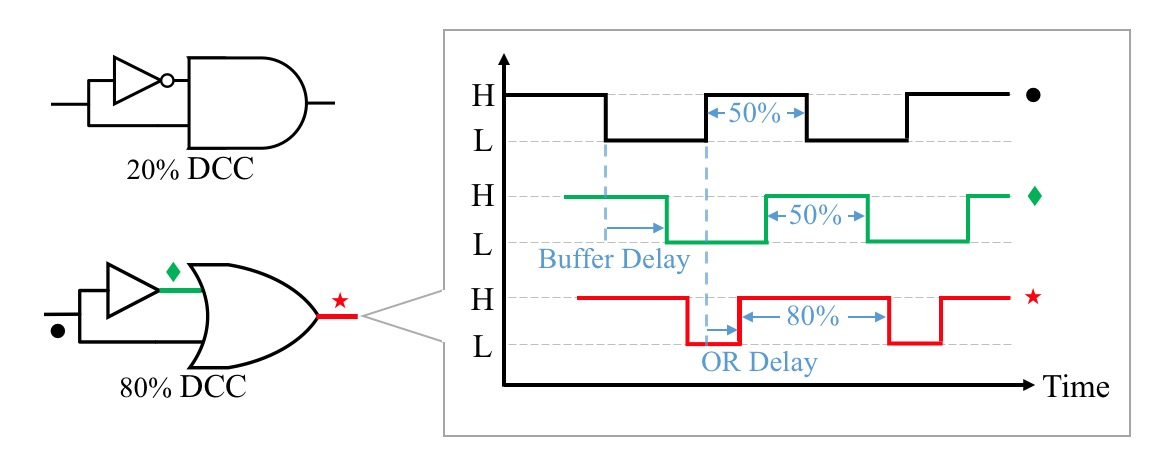
\includegraphics[width=1\columnwidth]{dcc.png}
    \caption{Construction of DCC and duty cycle transformation}
    \label{fig:dcc}
\end{figure}

\begin{figure}
    \centering
    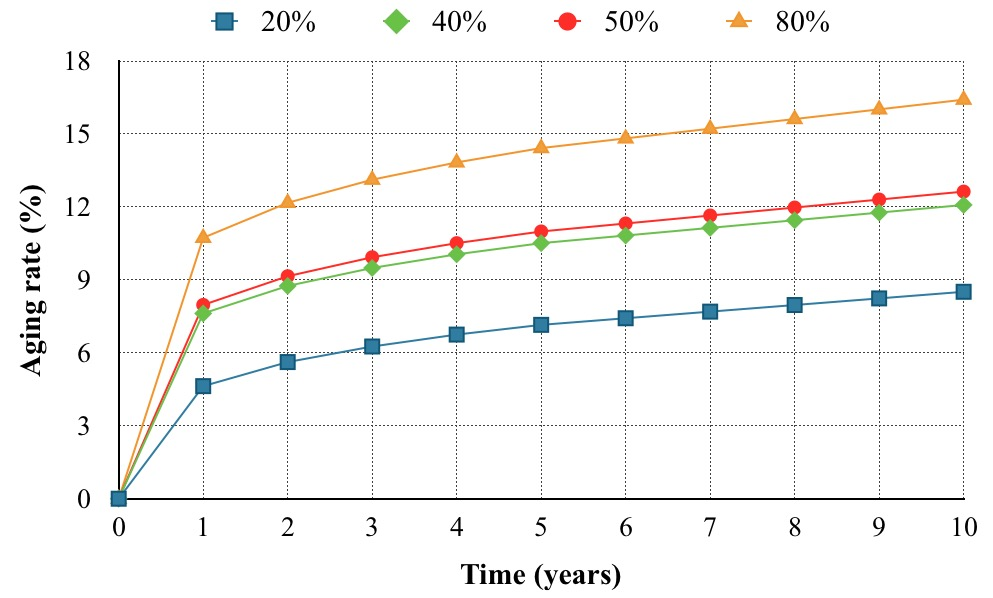
\includegraphics[width=1\columnwidth]{agr.png}
    \caption{Aging rates of buffers receiving different clock duty cycles}
    \label{fig:agr}
\end{figure}

Duty cycle is the percentage of one period in which a signal is high (i.e., logic 1). The aging of logic gates highly depends on the stress time~\cite{wang2010impact}. For a clock buffer on the clock tree, its stress time is proportional to the clock duty cycle. Therefore, by adjusting the clock duty cycle, we can manipulate the aging of clock buffers and then control the effective degradation of logic paths. Figure~\ref{fig:agr} shows the aging rates of clock buffers receiving different clock duty cycles. 

The unit we use to change the clock duty cycle is duty-cycle converter (DCC), which can converts the duty cycle of a clock signal to a smaller/larger one (e.g., $50\% \rightarrow 20\%$ or $50\% \rightarrow 80\%$), as shown in Figure~\ref{fig:dcc}. It separates the source clock wave (black line) and original wave. Then, the two waves are combined with the OR gate to obtain a new wave (red line) of 80\% duty cycle. Once a DCC is inserted into the clock tree, the downstream sub-tree of the DCC insertion point will receive a clock signal whose duty cycle is no longer 50\%. This way, aging rate manipulation of downstream clock buffers can be achieved.


\begin{figure}
    \centering
    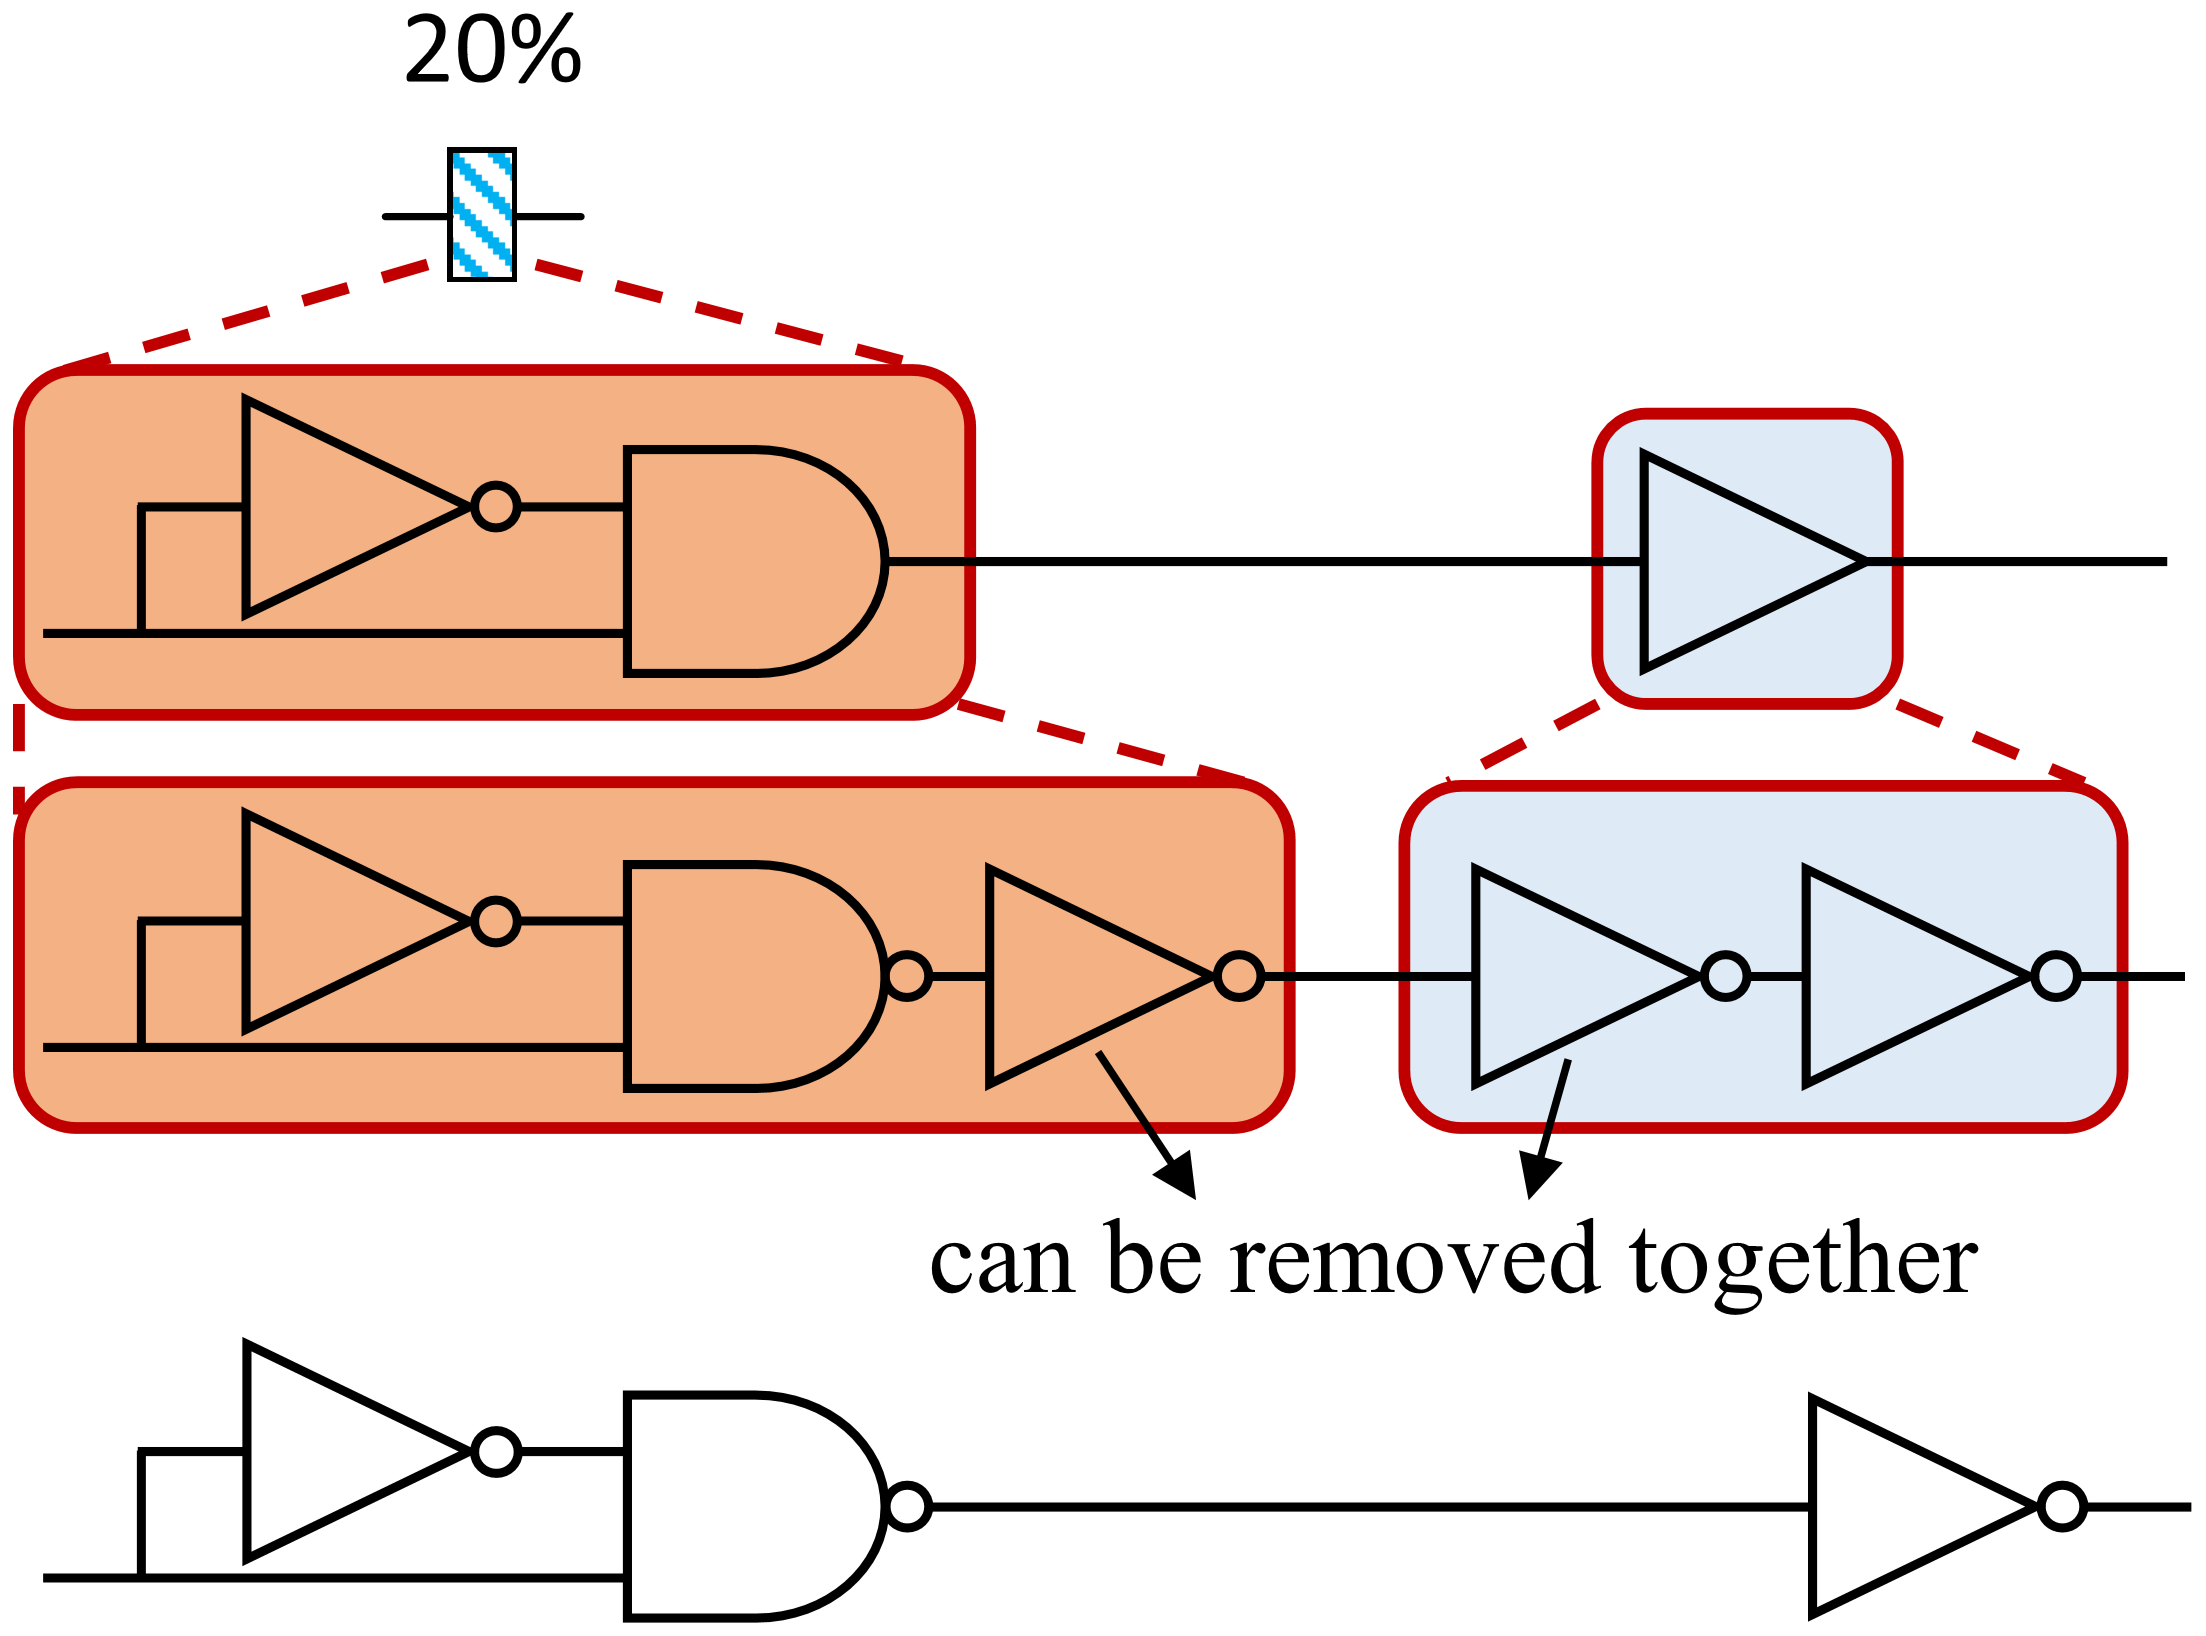
\includegraphics[width=0.5\columnwidth]{DCC_reduction.png}
    \caption{Practical considerations for DCC insertion}
    \label{fig:dccreduc}
\end{figure}

\subsection{Practical Considerations}
\label{subsec:tpc}
The diagram on the top of Figure~\ref{fig:dccreduc} shows the primitive design of a DCC, consisting of an inverter and an AND gate. In practice, the AND gate is implemented by a NAND gate feeding an inverter. As mentioned earlier, when inserting a DCC, it is inserted at the input of a buffer, which is a pair of inverters in practice. Therefore, we can actually use the diagram on the bottom of Figure~\ref{fig:dccreduc} to realize the insertion of a DCC. More specifically, we use it as a new cell to \enquote{replace} a buffer when a DCC is needed. By doing so, the cost of a single DCC can be significantly reduced and not much more expensive than the cost of inserting a buffer for clock skew scheduling. 

\section{PROPOSED FRAMEWORK}
\label{sec:framework}
In the proposed framework, aging tolerance is achieved by recycling useful/beneficial skews into the designs, based on the concept of timing borrowing. The beneficial skews are progressively created due to different aging behaviors of clock paths caused by DCCs. Moreover, high-$V_{th}$ assignment for clock buffers is also incorporated in the proposed framework to explore/recycle more beneficial skews, further improving aging tolerance of the designs.
The overall flow of our framework is depicted in Figure~\ref{fig:flow}, where we focus on the following three tasks:
\begin{enumerate}[leftmargin=*]
	\item \textbf{Minimization of clock period:} The clock period can be minimized since the performance degradation of the logic circuit is \enquote{tolerated} as a result of useful clock skews. The minimum required clock period thus implies maximum level of aging tolerance. As depicted in Figure~\ref{fig:flow}, a binary search for optimal clock period is involved in the proposed framework.
	\item \textbf{DCC deployment:} The problem of  DCC deployment is formulated as a Boolean Satisfiability (SAT) problem. Therefore, the key of our framework is to represent the problem in \textit{conjunctive normal form} (CNF). A CNF representation is a conjunction of one or more clauses, where each clause is a disjunction of one or more Boolean variables. Thanks to the efficiency of existing SAT solvers, the solution can be obtained efficiently. The end result of this formulation is the locations (in the existing clock tree) of DCCs, such that the required clock period of the given circuit under $n$-year BTI is minimized when aging-induced clock skews are considered. 
	\item \textbf{High-$V_{th}$ assignment for clock buffers:} The problem of high-$V_{th}$ assignment for clock buffers is also formulated as a SAT-based problem, represented in CNF and solved by existing SAT solvers.
\end{enumerate}
\begin{figure}
	%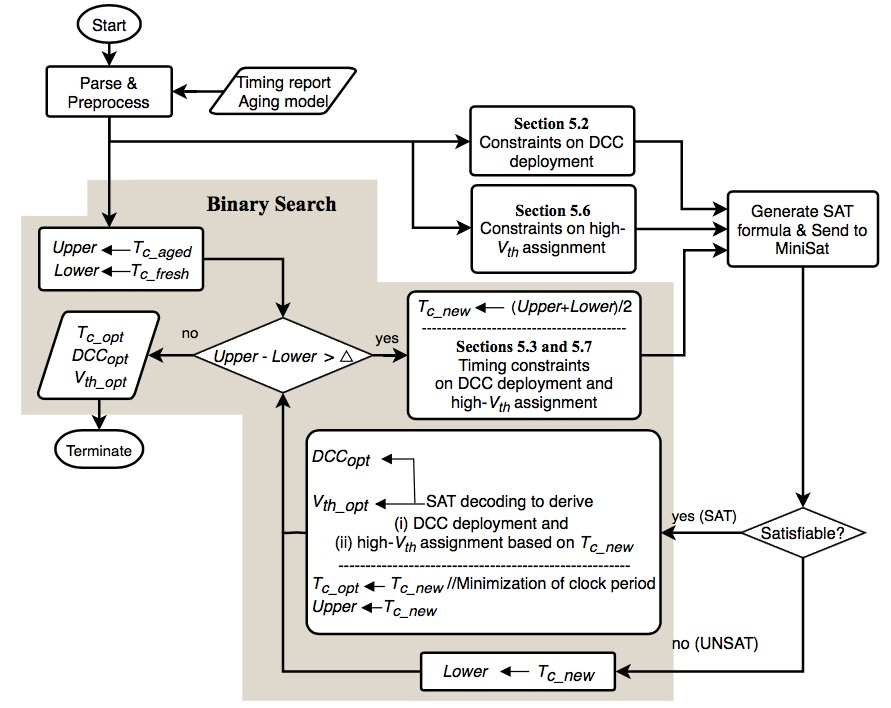
\includegraphics[width=1\columnwidth]{Flow_chart.png} %IEEE Journal
	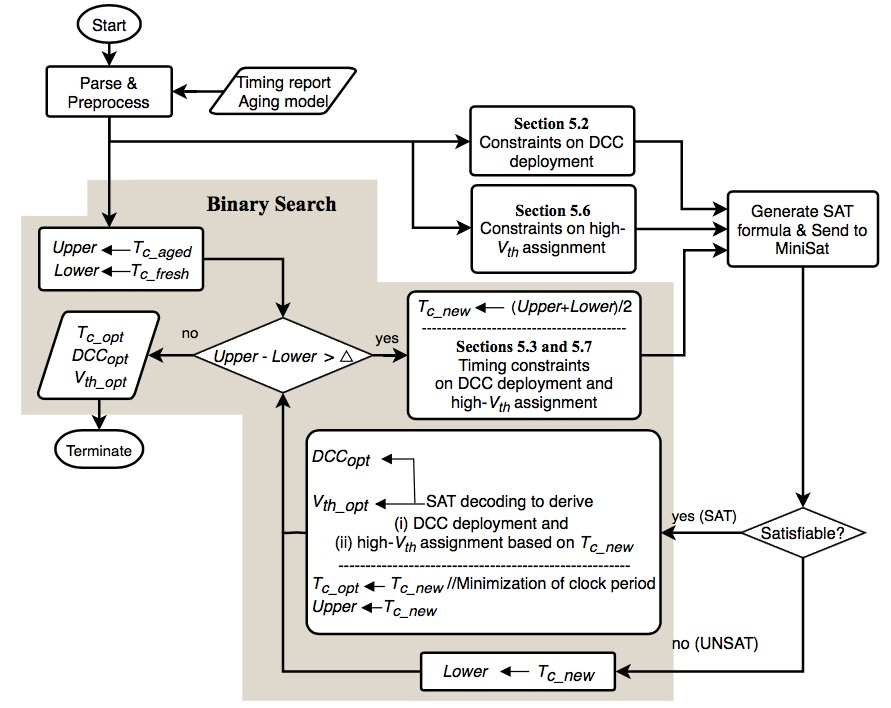
\includegraphics[width=0.85\columnwidth]{Flow_chart.png} %ACM Journal
	\caption{The overall flow of MAUI}
	\label{fig:flow}
\end{figure}
 
 This section is organized as follows: Section~\ref{subsec:eddcd} explains how the proposed problem of DCC deployment/insertion are encoded into Boolean variables. Section~\ref{subsec:dccccc} and Section~\ref{subsec:tccc} describe three major components, DCC constraints and timing constraints, for our SAT-based formulation and how they are translated into legal SAT formula, i.e., CNF representation. Finally, Sections~\ref{sec:VTA}-\ref{sec:VTA:timing} introduce the additive improvements by employing high-$V_{th}$ assignment on buffers.
\afterpage{ 
\begin{figure}
	\centering
	%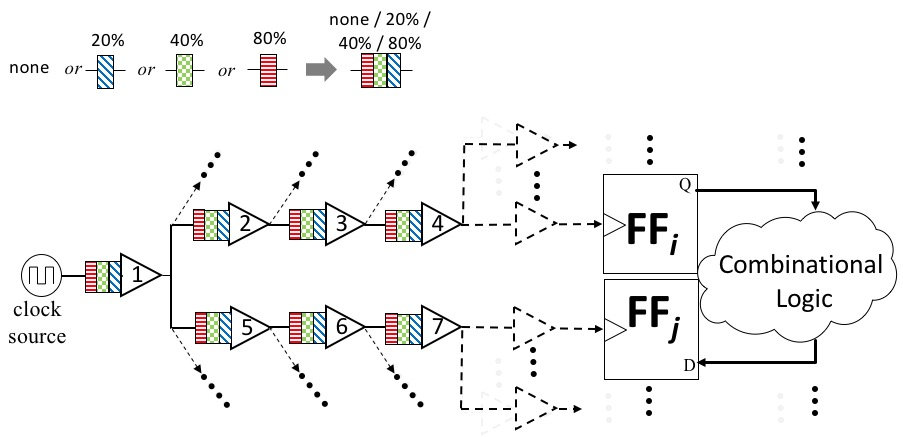
\includegraphics[width=1.0\columnwidth]{All_types_of_DCCs.png} %IEEE Journal
	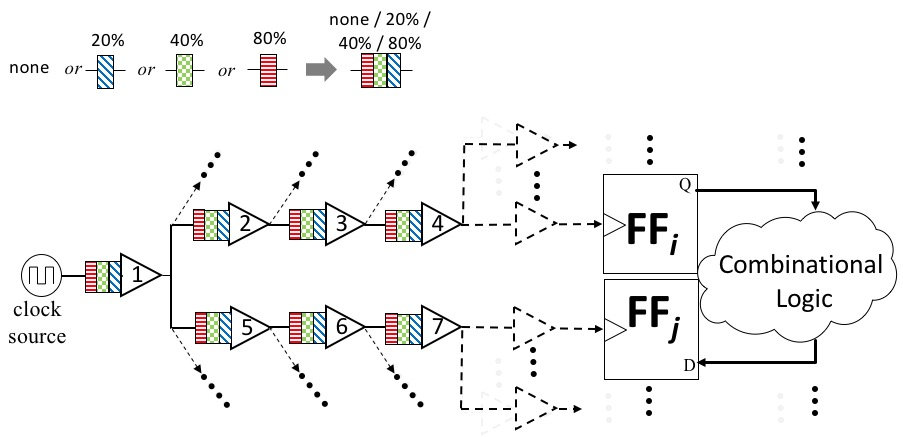
\includegraphics[width=0.7\columnwidth]{All_types_of_DCCs.png} %ACM Journal
	\caption{Generalized DCC insertion for a target pair of flip-flops} 
	\label{fig:dcctype} 
\end{figure}
}

%(3) DATE 2018
\subsection{Boolean Encoding for DCC Deployment}
\label{subsec:eddcd}
The problem of DCC deployment needs to be encoded into Boolean representation before being transformed into a SAT-based formulation. Assume that a total of $N$ types of DCCs can be chosen. Including the DCC-free case where no DCC is inserted, there are ($N$ + 1) possibilities of DCC insertion for each clock buffer. We denote a clock buffer by $p\left(1 \leq p \leq P\right)$ where $P$ is the total count of clock buffers and $p$ is buffer index. For each clock buffer, there exist two types of Boolean variables, {\fontsize{9}{10}$B_{p,q}$} ($1 \leq q \leq Q $, $Q = \lceil \lg (N + 1)\rceil$), where {\fontsize{9}{10}$\left\{B_{p,1}, B_{p,2},\dotsc, B_{p,Q}\right\}$} encode the aforementioned ($N$ + 1) possibilities of DCC insertion at the input of buffer $p$.

Without loss of generality, we assume $N$ = 3. Thus, there are three types of DCCs, assumed to be 20\%, 40\%, and 80\% DCCs, as shown in Figure~\ref{fig:dcctype}. Therefore, three Boolean variables are used for encoding 4 possibilities of DCC at any buffer. The 4 possibilities can be encoded as follows:

%(5) DATE 2018
{\small
\begin{tabular}{ c c c }
\centering
   & DCC type & $\left\{B_{p,2},B_{p,1}\right\}$ \\
  (1)\quad & None & \{0, 0\} \\
  (2)\quad & 20\% &  \{0, 1\} \\
  (3)\quad & 40\% &  \{1, 0\} \\
  (4)\quad & 80\% &  \{1, 1\} \\
\end{tabular}}

\afterpage{
\begin{figure*}
    \centering
    \subfigure[Class 2-1: one DCC on the common clock path (e.g., at buffer 1)]{
    	\label{fig:sub:dcci1}
        %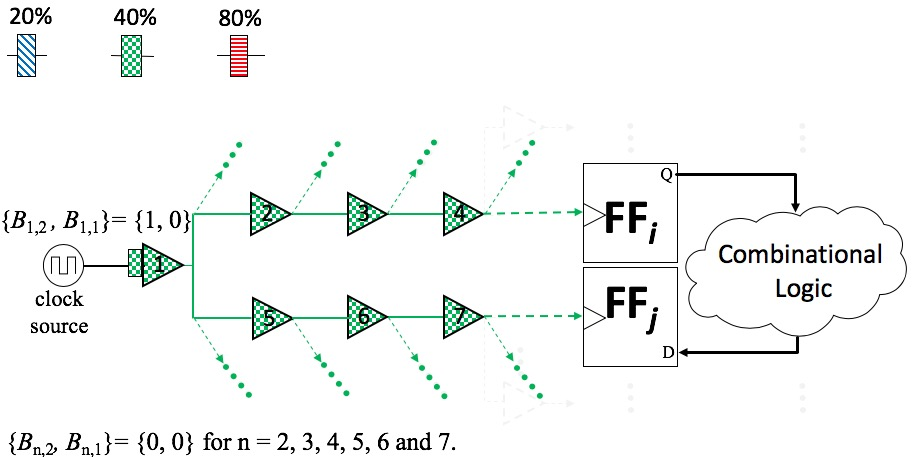
\includegraphics[width=0.92\columnwidth]{A_examlpe_of_DCC_placement1.png}  %IEEE Journal
        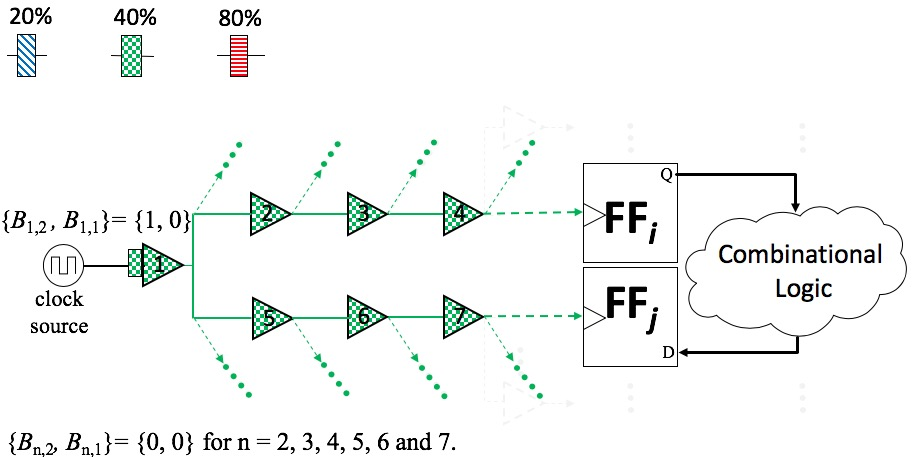
\includegraphics[width=0.65\columnwidth]{A_examlpe_of_DCC_placement1.png}  %ACM Journal
    }
    \hspace{1cm}
    \subfigure[Class 2-2: one DCC on one of the divergent clock paths, or class 3: two DCCs, one on each of the divergent clock paths]{
    	\label{fig:sub:dcci2}
        %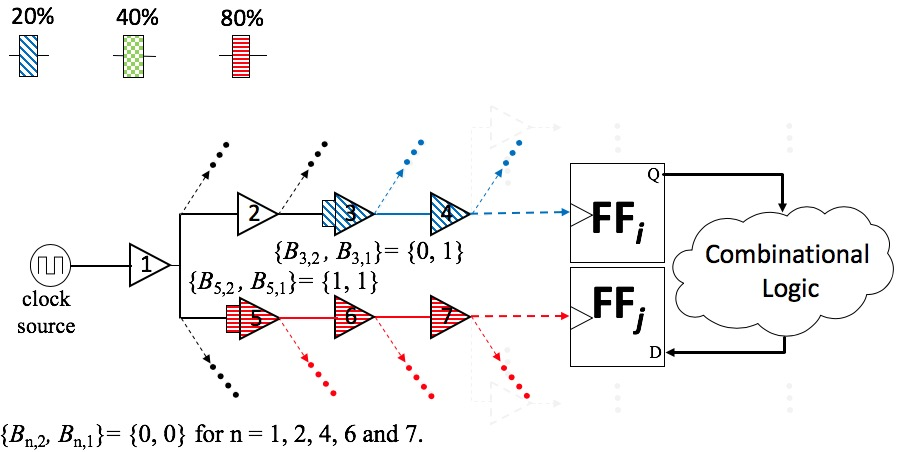
\includegraphics[width=0.92\columnwidth]{A_examlpe_of_DCC_placement2.png}  %IEEE Journal
        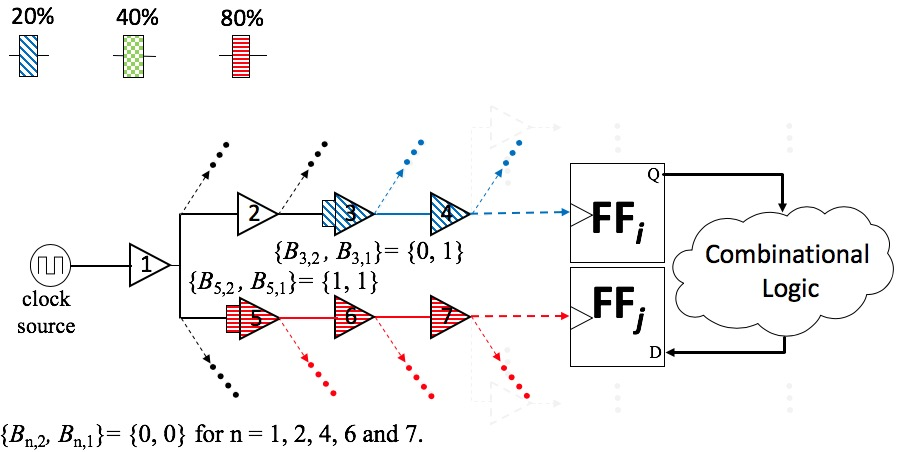
\includegraphics[width=0.65\columnwidth]{A_examlpe_of_DCC_placement2.png}  %ACM Journal
    }
    \caption{Examples of DCC insertion}
    \label{fig:dccinsert}
\end{figure*}
}


For example, in Figure~\ref{fig:sub:dcci2}, a 20\% DCC and an 80\% DCC are inserted at buffer 3 and buffer 5, respectively. Therefore, {\fontsize{9}{10}{$\left\{B_{3,2}, B_{3,1}\right\}$ = \{0, 1\}}}, {\fontsize{9}{10}{$\left\{B_{5,2}, B_{5,1}\right\}$ = \{1, 1\}}}, and {\fontsize{9}{10}{$\left\{B_{p,2}, B_{p,1}\right\}$ = \{0, 0\}}} for $p$ = 1, 2, 4 , 6 or 7.

The 20\% DCC will mitigate the aging of buffer 3 and its downstream buffers, while the 80\% DCC will aggravate the aging of buffer 5 and its downstream buffers. It can be found that, if a DCC is deployed deep in the clock tree (i.e., close to the flip-flops), the count of affected buffers is limited and thus the overall impact of aging mitigation/aggravation on $C_i$/$C_j$ may be insignificant, diminishing the benefit from deploying DCCs for aging tolerance.  To avoid the phenomena, we set a rule of prohibiting DCC deployment at a clock tree level larger/deeper than a specified boundary. This rule also greatly reduces the complexity of our SAT-based formulation because a significant fraction of buffers are excluded from being considered inserted DCC at their inputs. For example, in Figure~\ref{fig:dcctype}, those dashed buffers and their downstream buffers are excluded. 

%(2) B
\subsection{Constraints on DCC Deployment}
\label{subsec:dccccc}
Figure~\ref{fig:dcctype} shows a generalized example of DCC insertion for a pair of flip-flops (\ce{FF_i} and \ce{FF_j}) where there exist \textit{aging-critical paths} from \ce{FF_i} to \ce{FF_j}, defined as follow:\\

\noindent \textbf{\uline{Definition 1} (\textit{Aging-critical path}):}  A path is defined as an \textit{aging-critical path} if, in the presence of aging, it is possible to determine the clock period of the circuit.\\ 

Every pair of flip-flops between which there exist aging-critical paths needs to be considered and here, we use this generalized example to illustrate our SAT-based formulation. In Figure~\ref{fig:dcctype}, buffers 1 - 7 are candidate locations for DCC insertion and according to the encoding scheme explained in Section~\ref{subsec:eddcd}, two Boolean variables are introduced for each of the seven buffers to encode four possibilities of DCC insertion. Considering all seven buffers, there are a total of 16,384 (= $4^7$) possibilities for DCC insertion, just for this pair of flip-flops. This makes the SAT-based formulation intractable due to the explosion of clause count. Therefore, we set up the following constraints on DCC insertion: \\

\noindent \textbf{\uline{Constraint 1} (\textit{DCC constraint}):} At most one DCC on a single clock path (from the clock source to one of the flip-flops).\\

In order to ensure no more than one DCC on any clock path, we can use the Boolean variables introduced for DCC insertion, i.e., {\fontsize{9}{10}$B_{p,q} \left(1 \leq p \leq P, 1 \leq q \leq Q = \lceil \lg (N + 1) \rceil \right)$}, to generate some clauses which suppress the occurrence of having two DCCs on a clock path. Consider buffer 2 (encoded by {\fontsize{9}{10}$\left\{B_{2,2}, B_{2,1}\right\}$}) and buffer 3 (encoded by {\fontsize{9}{10}$\left\{B_{3,2}, B_{3,1}\right\}$}) in Figure~\ref{fig:dcctype}. If there is a DCC at buffer 2 (i.e., {\fontsize{9}{10}$\{B_{2,2}, B_{2,1}\} \not\equiv \{0, 0\}$}), then there must no DCC at buffer 3 (i.e., {\fontsize{9}{10}$\{B_{3,2}, B_{3,1}\} \equiv \{0, 0\}$}), and vice versa. The constraint can be formally written as:
{\fontsize{9}{10}
\begin{gather*}
\left(\{B_{2,2}, B_{2,1}\} \equiv \{0, 0\}\right) \lor \left(\{B_{3,2}, B_{3,1}\} \equiv \{0, 0\}\right)
\end{gather*}}
Next, it can be translated into 4 CNF clauses:
{\fontsize{9}{10}
\begin{equation*}
\begin{split}
(\neg B_{2,1}\lor\neg B_{3,1}) \land (\neg B_{2,1}\lor\neg B_{3,2}) \land (\neg B_{2,2}\lor\neg B_{3,1}) \land (\neg B_{2,2}\lor\neg B_{3,2})
\end{split}
\end{equation*}}
Any pair of buffers along a single clock path should be constrained in this way. Among buffers 1- 7 in Figure~\ref{fig:dcctype}, there are 12 pairs: $\langle1, 2\rangle$, $\langle1, 3\rangle$, $\langle1, 4\rangle$, $\langle1, 5\rangle$, $\langle1, 6\rangle$, $\langle1, 7\rangle$, $\langle2, 3\rangle$, $\langle2, 4\rangle$, $\langle3, 4\rangle$, $\langle5, 6\rangle$, $\langle5, 7\rangle$, $\langle6, 7\rangle$. Each pair translates to 4 clauses and a total of 48 clauses will be generated accordingly.

With DCC constraints and corresponding clauses, we can drastically reduce the possibilities of DCC insertion to be formulated. In the above example where the 48 clauses associated with DCC constraints are generated, the possibility count of DCC insertion drops from 16,384 to 103. In the next subsection, we describe what the 103 possibilities are and how they are translated into the final CNF representation.

%(3) C
\subsection{Timing Constraints and Corresponding Clauses}
\label{subsec:tccc}
Given a pair of flip-flops, if there exists one logic path between them, the timing (i.e. setup-time and hold-time) constraints must be met based on the inequalities~(\ref{eq:tsu}) and~(\ref{eq:th}). Different types of DCCs reveal different influence on clock latency. Consider the lifespan specification of 10 years in Figure~\ref{fig:sub:dcci2}: the delay of each clock buffer is changed after 10 years. The clock latency of \ce{FF_i} (i.e., $C_i$) is the sum of clock buffer delays from clock source to \ce{FF_i}: 
\begin{gather*}
C_i = \tau_1 + \tau_2 + \tau_3 + \tau_4 +\dotsb \\
C_j = \tau_1 + \tau_5 + \tau_6 + \tau_7 +\dotsb
\end{gather*}
where $\tau_k$ is the delay of buffer $k$. Consider aging effects on $C_i$ and $C_j$: 
\begin{gather*}
C_{i\_aged} = 1.13 \times \left(\tau_1 + \tau_2\right) + 1.09 \times \left(\tau_3 + \tau_4 + \dotsb\right)\\
C_{j\_aged} = 1.13 \times \tau_1+ 1.16 \times \left( \tau_5 + \tau_6 + \tau_7 + \dotsb \right)
\end{gather*}
where $C_{i\_aged}$ and $C_{j\_aged}$ denote aged $C_i$ and $C_j$, respectively. Next, we apply Equations~(\ref{eq:tsu}) and~(\ref{eq:th}) to check whether timing constraints will be violated under this DCC deployment.\\

\noindent \textbf{\uline{Constraint 2} (\textit{Timing constraint}):} No existence of timing violation.\\

Given one clock period $T_c$ derived by binary search, one aging-critical path, and its associated clock network, all possible DCC deployment can be classified into 3 classes according to the number of DCCs used. Furthermore, due to the aforementioned DCC constraints, the SAT solver will only output a DCC deployment where there does not exist more than one DCC along any clock path. Thus, in the following discussion, the deployment with more than one DCC along a single clock path can be ignored. In each class, if the DCC deployment causes a timing violation within 10 years (i.e., the lifespan specification), then the deployment will be transformed into CNF clauses, such that the solver will not output the deployment as results. Here, we explain the generation of CNF clauses by using the example in Figure~\ref{fig:dccinsert}.\\

\noindent \textbf{Class 1:} No DCC is inserted on either clock path

Consider the situation that no DCC is inserted at buffers 1- 7. If it causes a timing violation along the aging-critical path within 10 years, then the Boolean representation of the deployment,
{\fontsize{9}{10}
\begin{gather*}
\left(\{B_{1,2}, B_{1,1}\} \equiv \{0, 0\} \right) \land \left( \{B_{2,2}, B_{2,1}\} \equiv \{0, 0\} \right) \land \dotsb 
\land \left( \{B_{7,2}, B_{7,1}\} \equiv \{0, 0\} \right),
\end{gather*}}
equivalent to the following CNF clause:
{\fontsize{9}{10}
\begin{gather*}
\left(B_{1,2} \lor B_{1,1} \lor B_{2,2} \lor B_{2,1} \lor \dotsb \lor B_{7,2} \lor B_{7,1} \right),
\end{gather*}}
should be generated such that the solver will not output the corresponding deployment in the result if the CNF is satisfiable. In this case, a total of 1 CNF clause is generated.\\

\noindent \textbf{Class 2:} Inserting one DCC

This class can be further classified into 2 sub-classes based on the location of inserted DCCs. \\
\textit{Class 2-1:} Inserting one DCC on the common clock path
In Figure~\ref{fig:dccinsert}, buffer 1 is on the common clock path. Consider the DCC insertion shown in Figure~\ref{fig:sub:dcci1}: if the insertion of a 40\% DCC at buffer 1 causes a timing violation within 10 years, then the Boolean representation of the DCC deployment,
{\fontsize{9}{10}
\begin{gather*}
\left(\{B_{1,2}, B_{1,1}\} \equiv \{1, 0\} \right) \land \left( \{B_{2,2}, B_{2,1}\} \equiv \{0, 0\} \right) \land \dotsb 
\land \left( \{B_{7,2}, B_{7,1}\} \equiv \{0, 0\} \right),
\end{gather*}}equivalent to the following clause:
{\fontsize{9}{10}
\begin{gather*}
\left(\neg B_{1,2} \lor B_{1,1} \lor B_{2,2} \lor B_{2,1} \lor \dotsb \lor B_{7,2} \lor B_{7,1} \right),
\end{gather*}}should be generated such that the solver will not output the deployment in the result if the CNF is satisfiable. Given that there are 3 choices of DCCs, a total of 3 CNF clauses will be generated in the worst case. \\
\textit{Class 2-2:} \mbox{\fontsize{9}{10.8}\selectfont Inserting one DCC on one of the divergent clock paths}

This class targets buffers 2, 3, 4, 5, 6, 7. If the insertion of a 20\% DCC at buffer 3 causes a timing violation within 10 years, then the Boolean representation of the DCC deployment, 
{\fontsize{9}{10}
\begin{gather*}
	\left(\{B_{3,2}, B_{3,1}\} \equiv \{0, 1\} \right) \land \left( \{B_{1,2}, B_{1,1}\} \equiv \{0, 0\} \right) \land \dotsb 
	\land \left( \{B_{7,2}, B_{7,1}\} \equiv \{0, 0\} \right),
\end{gather*}}equivalent to the following CNF clause:
{\fontsize{9}{10}
\begin{gather*}
	(B_{3,2} \lor \neg B_{3,1} \lor B_{1,2} \lor B_{1,1} \lor B_{2,2} \lor B_{2,1} \lor B_{3,2} \dotsb  
\lor B_{7,2} \lor B_{7,1}),
\end{gather*}}should be generated such that the solver will not output the deployment in the result if the CNF is satisfiable. This class includes 6 candidates: buffers 2, 3, 4, 5, 6, 7, and each has 3 choices of DCCs. Therefore, a total of 18 CNF clauses will be generated in the worst case.\\

\noindent \textbf{Class 3:} Inserting two DCCs on two clock paths respectively

Given the DCC deployment in Figure~\ref{fig:sub:dcci2} (a 20\% DCC inserted at buffer 3 and a 80\% DCC inserted at buffer 5), if it causes a timing violation along the aging-critical path within 10 years, then the Boolean representation of the deployment,
{\fontsize{9}{10}
\begin{gather*}
\left(\{B_{1,2}, B_{1,1}\} \equiv \{0, 0\} \right) \land \left(B_{2,2}, B_{2,1}\} \equiv \{0, 0\} \right) \land \left(\{B_{3,2}, B_{3,1}\} \equiv \{0, 1\} \right) \\ 
\land \left( \{B_{4,2}, B_{4,1}\} \equiv \{0, 0\} \right) \land \left(\{B_{5,2}, B_{5,1}\} \equiv \{1, 1\} \right) \land \left( \{B_{6,2}, B_{6,1}\} \equiv \{0, 0\} \right)\\
\land \left( \{B_{7,2}, B_{7,1}\} \equiv \{0, 0\} \right),
\end{gather*}}equivalent to the following CNF clause,
{\fontsize{9}{10}
\begin{gather*}
(B_{1,2} \lor B_{1,1} \lor B_{2,2} \lor B_{2,1} \lor B_{3,2}  \lor \neg B_{3,1} \lor B_{4,2} \lor B_{4,1} \lor \neg B_{5,2} \lor \neg B_{5,1} \lor B_{6,2} \lor B_{6,1} \lor B_{7,2} \lor B_{7,1} )
\end{gather*}}should be generated such that the solver will not output the deployment in the result if the CNF is satisfiable.

Class 3 considers two buffer locations to insert DCCs, one among buffers \{2, 3, 4\} and the other one among buffers \{5, 6, 7\}; thus, there are totally 9 combinations of buffer locations. Each combination includes two buffers and thus 9 possibilities of choosing one specific DCC for each of the two buffers. Therefore, a total of 81 CNF clauses will be generated in the worst case.

Considering all of the above cases, a maximum number of 1 + 3 + 18 + 81 = 103 clauses can be derived. This is based on the existence of 48 clauses introduced in Section~\ref{subsec:dccccc}.

\subsection{Additive Improvement in Aging Tolerance: High-$V_{th}$ Assignment for Clock Buffers}
\label{sec:VTA}
Aging tolerance is achieved by exploring/recycling useful aging-induced clock skews, based on the concept of timing borrowing. So far, the useful skews can be progressively created due to different aging behaviors of clock paths caused by inserting 20\%, 40\% and 80\% DCCs in the existing synthesized clock network. In order to enhance the benefit of useful aging-induced skews, the technique of high-$V_{th}$ assignment for clock buffers, an additive methodology for aging tolerance, is incorporated in our framework. In this way, the exploration space of our optimization framework based on useful skews is enlarged, such that more useful skews can be recycled, enhancing our idea of making aging useful. In the following subsections, the techniques of DCC deployment and high-$V_{th}$ assignment for clock buffers are jointly integrated.

Such a technique of high-$V_{th}$ assignment can cause an issue of fragmentary high-$V_{th}$ assignment for clock buffers. That is, the $V_{th}$ values of continuous buffers along a clock path interlace between high and nominal value. It may decrease the feasibility/manufacturability of the proposed framework. In order to avoid such a phenomenon, we set a rule:\\

\textit{Along a clock path, if the $V_{th}$ value of a clock buffer is assigned high value, then the $V_{th}$ values of its downstream buffers must be also assigned high value.}\\

Such a rule can suppress the occurrence of fragmentary high-$V_{th}$ assignment for clock buffers. Moreover, it also transforms the problem of high-$V_{th}$ assignment to the problem of selecting \textit{high-$V_{th}$ buffer leader}, which is defined as follow:\\

\noindent \textbf{\uline{Definition 2} (\textit{High-$V_{th}$ buffer leader}):} A clock buffer is defined as a \textit{high-$V_{th}$ buffer leader}, if the $V_{th}$ values of its downstream buffers (include the leader itself) are assigned high value and the $V_{th}$ values of its upstream buffers (exclude the leader itself) are nominal value.\\

Conceptually, there exists one difference between DCCs and high-$V_{th}$ buffer leaders. DCCs are physical gates inserted at the inputs of clock buffers to manipulate the aging rates of downstream buffers. However, high-$V_{th}$ buffer leaders, selected from the existing clock buffers, indicate where we begin assigning high $V_{th}$ to the buffers toward flip-flops (exclusive).

\subsection{Boolean Encoding for high-$V_{th}$ Buffer Leaders and DCCs}
The problem of selecting high-$V_{th}$ buffer leaders is also formulated as a SAT-based problem, solved by existing SAT solver, as we do for DCC deployment. The end result of the formulation involves the selected clock buffers (as leaders) and locations of DCCs. Assume that there are three types of DCCs (20\%, 40\%, and 80\%) and one type of high-$V_{th}$ buffer leader. Therefore, three Boolean variables are used for encoding 8 possibilities of DCC insertion and leader selection at any buffer. Consider the clock buffer $p$, the 8 possibilities can be encoded as follows:
{\small
\begin{tabular}{  c  c  c  c  }
  	 & Leader or not & DCC type & $\{B_{p,3}, B_{p,2}, B_{p,1}\}$ \\ 
  	(1)\quad & No & None & \{0, 0, 0\} \\ 
  	(2)\quad & No &20\% &  \{0, 0, 1\} \\ 
  	(3)\quad & No &40\% &  \{0, 1, 0\} \\ 
  	(4)\quad & No &80\% &  \{0, 1, 1\} \\ 
	(5)\quad & Yes & None & \{1, 0, 0\} \\ 
  	(6)\quad & Yes & 20\% &  \{1, 0, 1\} \\ 
  	(7)\quad & Yes & 40\% &  \{1, 1, 0\} \\ 
  	(8)\quad & Yes & 80\% &  \{1, 1, 1\} \\ 
\end{tabular}}

\noindent where \{$B_{p,2}, B_{p,1}$\} are used to encode 4 possibilities of DCC insertion at the input of buffer $p$, and \{$B_{p,3}$\} is used to encode 2 possibilities of leader selection for buffer $p$.
Note that, if the buffer, located deep in the clock tree, is selected as the leader, then the count of affected buffers is limited, diminishing the benefit from high-$V_{th}$ assignment for aging tolerance. Therefore, as we do for DCC deployment, we similarly set a rule of prohibiting selecting buffer leaders at a clock tree level larger/deeper than a specified boundary.
\subsection{Constraints on High-$V_{th}$ Assignment for Clock Buffers}
\begin{figure}[t!]
    \centering
    %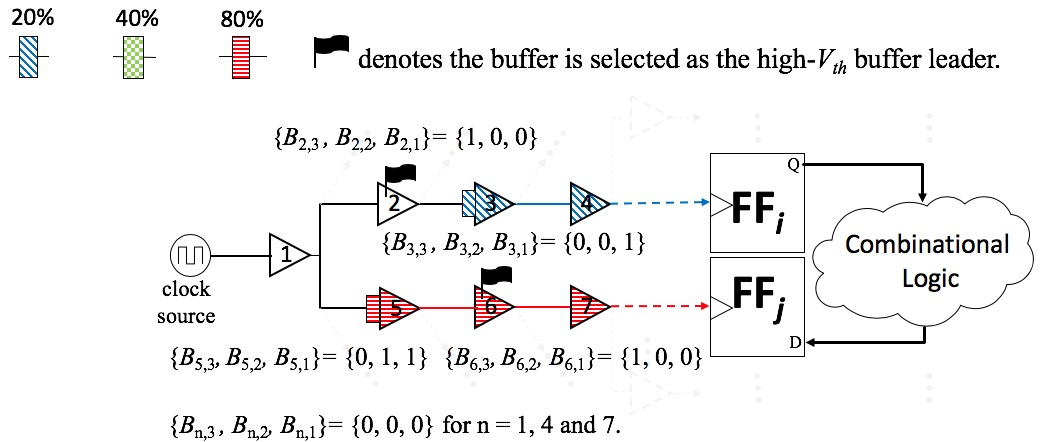
\includegraphics[width=1.0\columnwidth]{2DCC_2Leader.png} %IEEE
    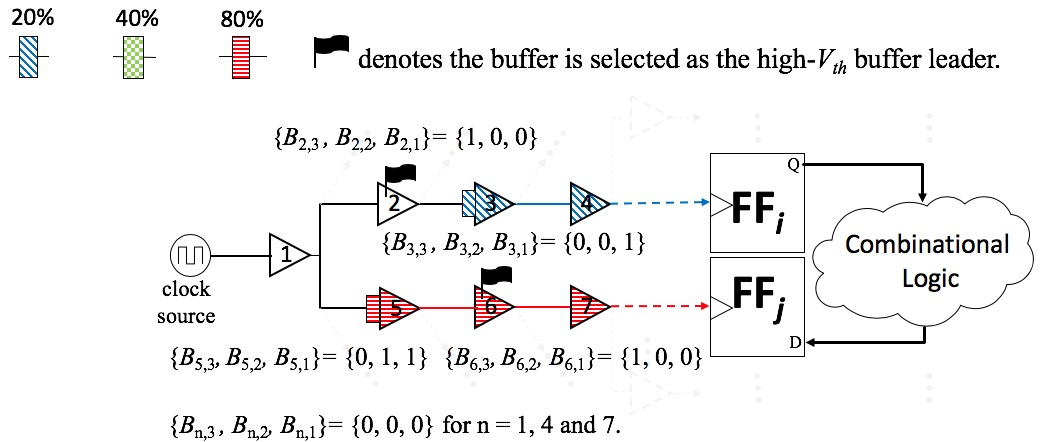
\includegraphics[width=0.71\columnwidth]{2DCC_2Leader.png} %ACM
    \caption{Example of DCC insertion and high-$V_{th}$ buffer leader selection}
    \label{fig:2dcc2leader}
\end{figure}

%Figure~\ref{fig:leadertype} shows a generalized example of DCC insertion and leader selection. It is worth reminding that, because of DCC constraints, the possibility count of DCC deployment has been dropped from 16,384 to 103. However, for each DCC deployment, there are still up to 128 ($2^7$) possibilities of leader selection, for this pair of flip-flops. Hence, we set up the following constraints on the selection of high-$V_{th}$ buffer leaders:

When two clock buffers along a single clock path are selected as leaders, the leader selection is meaningless, so that the following constraints are considered. In this way, the SAT solver will not output the corresponding leader selection in the result if the CNF is satisfiable.\\

\noindent \textbf{\uline{Constraint 3} (\textit{Leader constraint}):} At most one buffer along a single clock path is selected as high-$V_{th}$ buffer leader.\\
%\noindent \textbf{\uline{Leader constraint: At most one buffer along a single clock path is selected as high-$V_{th}$ buffer leader.}}

The constraint is similar to the aforementioned DCC constraint (see Section~\ref{subsec:dccccc}, Constraint 1). In order to ensure no more than one leader along any clock path, we generate some clauses to suppress the occurrence of having two leaders along a clock path. Consider buffer 2 (encoded by {\fontsize{9}{10}$B_{2,3}$}) and buffer 3 (encoded by {\fontsize{9}{10}$B_{3,3}$}) in Figure~\ref{fig:dcctype}. If buffer 2 is selected as a leader (i.e., {\fontsize{9}{10}${B_{2,3}} \equiv {1}$}), then buffer 3 must not be selected as a leader (i.e., {\fontsize{9}{10}$B_{3,3} \not\equiv {1}$}), and vice versa. The constraint can be formally written as:
{\fontsize{9}{10}
\begin{gather*}
\left(\{B_{2,3}\} \equiv \{1\}\right) \lor \left(\{B_{3,3}\} \equiv \{1\}\right)
\end{gather*}}
Next, it can be translated into 1 CNF clause:
{\fontsize{9}{10}
\begin{equation*}
\begin{split}
(\neg B_{2,3}\lor\neg B_{3,3})
\end{split}
\end{equation*}}
Any pair of buffers along a single clock path should be constrained in this way. Among buffers 1- 7 in Figure~\ref{fig:dcctype}, there are 12 pairs: $\langle1, 2\rangle$, $\langle1, 3\rangle$, $\langle1, 4\rangle$, $\langle1, 5\rangle$, $\langle1, 6\rangle$, $\langle1, 7\rangle$, $\langle2, 3\rangle$, $\langle2, 4\rangle$, $\langle3, 4\rangle$, $\langle5, 6\rangle$, $\langle5, 7\rangle$, $\langle6, 7\rangle$. Each pair translates to 1 clause and a total of 12 clauses will be generated accordingly.

With leader constraint and corresponding clauses, we can drastically reduce the possibilities of leader selection to be formulated. In the above example where the 12 clauses associated with leader constraint are generated, the possibility count of leader selection drops from 128 ($2^7$) to 17. Subsequently, the remaining 17 possibilities are considered in the timing constraints, introduced in the next subsection.

%------------------ Timing Constraints ()
\subsection{Timing Constraints Considering DCC Deployment and High-$V_{th}$ Assignment}
\label{sec:VTA:timing}
The timing constraints are similar to the former timing constraints (see Section~\ref{subsec:tccc}), while we here consider the influence of high-$V_{th}$ buffer leader on clock latency. It is worth reminding that, the former timing constraints are divided into 3 classes according to the used DCC count. Because we simultaneously consider the DCC deployment and leader selection in the existing clock network, each of the former 3 classes is further divided into 3 subclasses, in terms of the leader count (0, 1 and 2). Therefore, the timing constraints are divided into 9 ($3 \times 3$) subclasses, according to the used DCC count and leader count.

For simplicity, we make an illustrative example from one of the 9 subclasses: 2 DCCs and 2 high-$V_{th}$ buffer leaders in the clock network associated with aging-critical paths in Figure~\ref{fig:2dcc2leader}, where 20\% and 80\% DCC are inserted at the inputs of buffers 3 and 5, respectively, and buffers 2 and 6 are selected as high-$V_{th}$ buffer leaders, implying that the $V_{th}$ of buffer set \{2, 3, 4\} and buffer set \{6, 7\} are assigned high $V_{th}$ because of the leader buffer 2, 6, respectively. In the case, if it causes a timing violation along the aging-critical path, the Boolean representation of the DCC deployment and leader selection,
{\fontsize{9}{10}
\begin{gather*}
\left(\{B_{1,3}, B_{1,2}, B_{1,1}\} \equiv \{0, 0, 0\} \right) \land \left( \{B_{2,3}, B_{2,2}, B_{2,1}\} \equiv \{1, 0, 0\} \right) \land \left(\{B_{3,3}, B_{3,2}, B_{3,1}\} \equiv \{0, 0, 1\} \right) \\ 
\land \left( \{B_{4,3}, B_{4,2}, B_{4,1}\} \equiv \{0, 0, 0\} \right) \land \left(\{B_{5,3}, B_{5,2}, B_{5,1}\} \equiv \{0, 1, 1\} \right) \land \left( \{B_{6,3}, B_{6,2}, B_{6,1}\} \equiv \{1, 0, 0\} \right)\\
\land \left( \{B_{7,3}, B_{7,2}, B_{7,1}\} \equiv \{0, 0, 0\} \right),
\end{gather*}}equivalent to the following CNF clause:
{\fontsize{9}{10}
\begin{gather*}
(B_{1,3} \lor B_{1,2} \lor B_{1,1} \lor \neg B_{2,3} \lor B_{2,2} \lor B_{2,1}  \lor B_{3,3} \lor B_{3,2} \lor \neg B_{3,1} \lor B_{4,3} \lor B_{4,2} \\
\lor B_{4,1} \lor B_{5,3} \lor \neg B_{5,2} \lor \neg B_{5,1} \lor \neg  B_{6,3} \lor B_{6,2} \lor B_{6,1} \lor B_{7,3} \lor B_{7,2} \lor B_{7,1} )
\end{gather*}}should be generated such that the solver will not output the corresponding DCC deployment and leader selection in the result if the CNF is satisfiable. In this case, a total of 1 CNF clause is generated.

Note that, given the DCC deployment, if the leader count is 2, there exist 9 ($3 \times 3$) possibilities of leader selection (one among buffers $\{2, 3, 4\}$, the other one among buffers $\{5, 6, 7\}$). If the leader count is 1/0, there exist 7/1 possibilities of leader selection. Hence, there totally exist 17 ($9+7+1$) possibilities of leader selection, for each DCC deployment.




\section{EXPERIMENTAL SETTING, RESULTS AND DISCUSSION}
\label{sec:exp}
\subsection{Experimental Setting}
The proposed framework for aging tolerance is implemented in C++ and the SAT-based formulation is solved by MiniSat on a 2.83GHz Intel Quad-Core CPU workstation running Linux. The benchmark circuits are chosen from the IWLS'05 and ISCAS'89 suites. The technology used is TSMC 45nm GP standard cell series.

Under 10-year BTI, the aging rates of clock buffers were obtained from HSPICE. The aging rates of clock buffers with duty cycles of 20\%, 40\%, 50\%, and 80\% are 8.51\%, 12.08\%, 13.51\%, and 16.41\% respectively and the aging rate of logic is obtained by using the predictive model presented in~\cite{wang2010impact},~\cite{wang2007efficient} (detailed in Section~\ref{subsec:apm}).


\begin{table*}
\centering
\caption{Benchmark information}
	%\begin{tabular}{l}
	%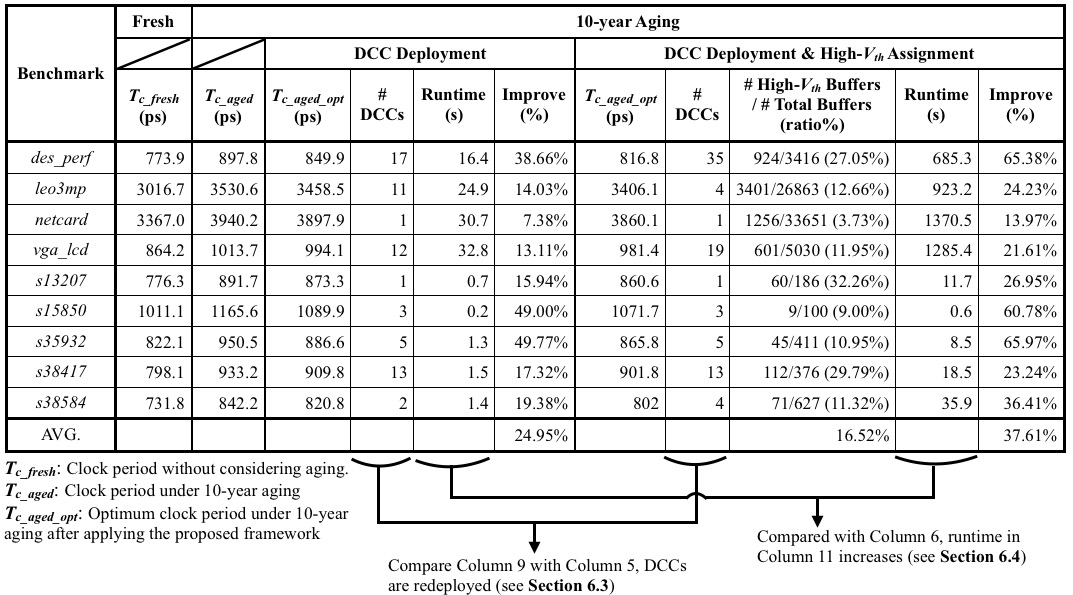
\includegraphics[width=2.03\columnwidth]{Experimental_result_DCC_TVA.png} %IEEE
	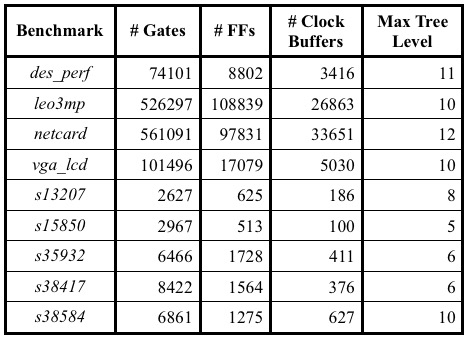
\includegraphics[width=0.47\columnwidth]{benchmark.png} %ACM
	%\end{tabular}
\label{table:exp1}
\end{table*}
\begin{table*}
\centering
\caption{Results of aging tolerance}
	%\begin{tabular}{l}
	%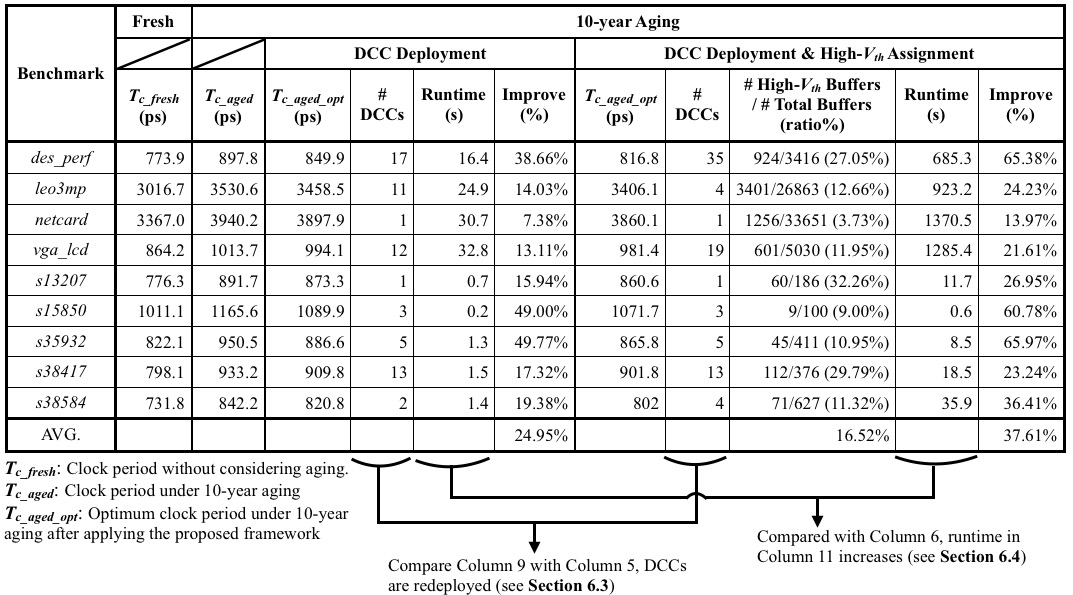
\includegraphics[width=2.03\columnwidth]{Experimental_result_DCC_TVA.png} %IEEE
	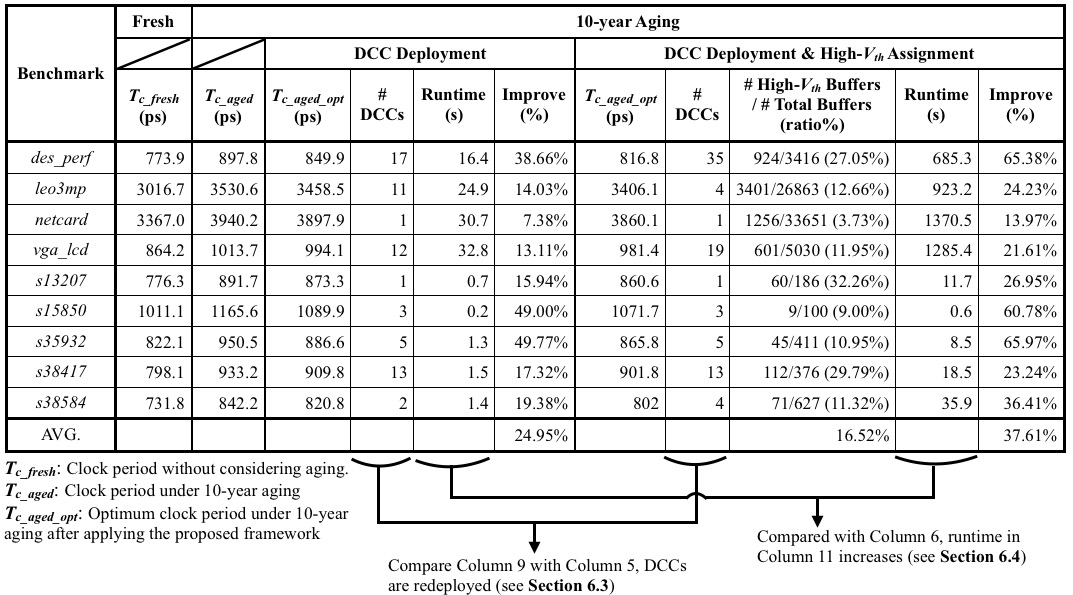
\includegraphics[width=1\columnwidth]{Experimental_result_DCC_TVA.png} %ACM
	%\end{tabular}
\label{table:exp2}
\end{table*}
\subsection{Experimental Results}
Table~\ref{table:exp1} and Table~\ref{table:exp2} reports the experimental results and information of each benchmark. In Table~\ref{table:exp1}, columns 2 to 5 show the total number of gates, total numbers of flip-flops, total numbers of clock buffers, and maximum level of the clock tree in each benchmark respectively. In Table~\ref{table:exp2}, column 2 demonstrates the fresh clock period that is the circuit delay without aging, denoted by $T_{c\_fresh}$. Column 3 demonstrates the clock period of the circuit under 10-year aging, denoted by $T_{c\_aged}$. Column 4 demonstrates the optimum clock period of the circuit under 10-year aging after applying our framework, denoted by $T_{c\_aged\_opt}$. A shorter clock period under aging implies better circuit performance and higher level of aging tolerance. Column 5 demonstrates the used DCC count. Column 6 demonstrates the runtime and the Column 7 demonstrates the improvement, i.e., the level of aging tolerance which is calculated as:
\begin{gather*}
1 - (T_{c\_aged\_opt} - T_{c\_fresh}) / (T_{c\_aged} - T_{c\_fresh})
\end{gather*}

For benchmark \textit{des\_perf}, $T_{c\_fresh}$ is 773.9ps and $T_{c\_aged}$ is 897.8ps, which means after 10-year aging the clock period of circuit will increase by 123.9ps. With DCC insertion using the proposed framework, the clock period achieved is 849.9ps, an increment of 76ps against $T_{c\_fresh}$ (38.66\% improvement). As shown in Table~\ref{table:exp2}, the improvement ranges from 7.38\% to 49.77\% and is 24.95\% on average. \iffalse As shown in Table~\ref{table:exp1}.\fi The number of inserted DCCs is between 2 (for benchmark \textit{s38584}) to 17 (for benchmark \textit{des\_perf}), implying very limited degree of circuit modification and insignificant design overhead. Moreover, as it can be seen in Column 12 to 16, when high-$V_{th}$ assignment for clock buffers is incorporated in the proposed framework, the resulting framework can give rise to lower clock periods, implying better improvement in aging tolerance. 

\subsection{Discussion: DCC Redeployment due to High-$V_{th}$ Assignment}
As we can see, the DCC counts in Column 13 are different from those in Column 9, implying that DCCs are redeployed in the clock tree while high-$V_{th}$ assignment is incorporated in the framework. More specifically, when high-$V_{th}$ assignment is considered, some clock buffers become candidate buffers to be inserted DCCs at their inputs, because timing constraints (i.e., setup-time and hold-time) are met based on the inequality Equation~(\ref{eq:tsu}) and (\ref{eq:th}). In this way, DCCs can be redeployed to obtain lower clock periods, exploring better improvement in aging tolerance.


%Compare the DCC counts in Column 9 with those in Column 13, we can find that, while $V_{th}^h$ assignment is involved in the framework, it may redeploy the DCCs in the clock tree and thus results in different DCC count. Specifically speaking, when $V_{th}^h$ assignment is considered, some clock buffers become candidate buffers to be inserted DCCs at their inputs, because timing constraints (i.e., setup-time and hold-time) are met based on the inequality Equation (1) and (2). In this way, DCCs can be redeployed to obtain lower clock periods.

%Take \textit{des\_perf} for example, DCC count is 7; however, the DCC count increases to 33 after $V_{th}^h$ assignment is involved. The DCC counts of the same design differ because the DCC deployments are not identical anymore. Specifically speaking, when V\textsubscript{th} assignment is considered, some clock buffers become candidate buffers to be inserted DCC at their inputs, because timing constraints (i.e., setup-time and hold-time) are met based on the inequality Equation (1) and (2), such that DCC can be redeployed to obtain lower Tc. Thus, even thought the two frameworks target the identical benchmark, the DCC deployments/counts may differ. 

\subsection{Discussion: Increase in Runtime}
In addition, the run time of the framework, incorporating high-$V_{th}$ assignment, increases due to the possibility explosion of DCC deployment and leader selection. To be specific, given a pair of flip-flops and associated clock paths, we need to consider the various possibilities of leader selections, for each DCC deployment. Therefore, the total  count of DCC deployment and leader selection is equal to the combination of DCC deployment plus leader selection, i.e., DCC possibilities multiplied by the leader counterparts, accounting for the increase of run time. 

Even though the runtime increase while high-$V_{th}$ assignment is incorporated, the resulting framework is still practical for aging tolerance because it at most takes 1370 seconds for a comparative design (e.g., netcard).
\subsection{Discussion: Aging Impact on DCC}
\begin{figure}
    \centering
    %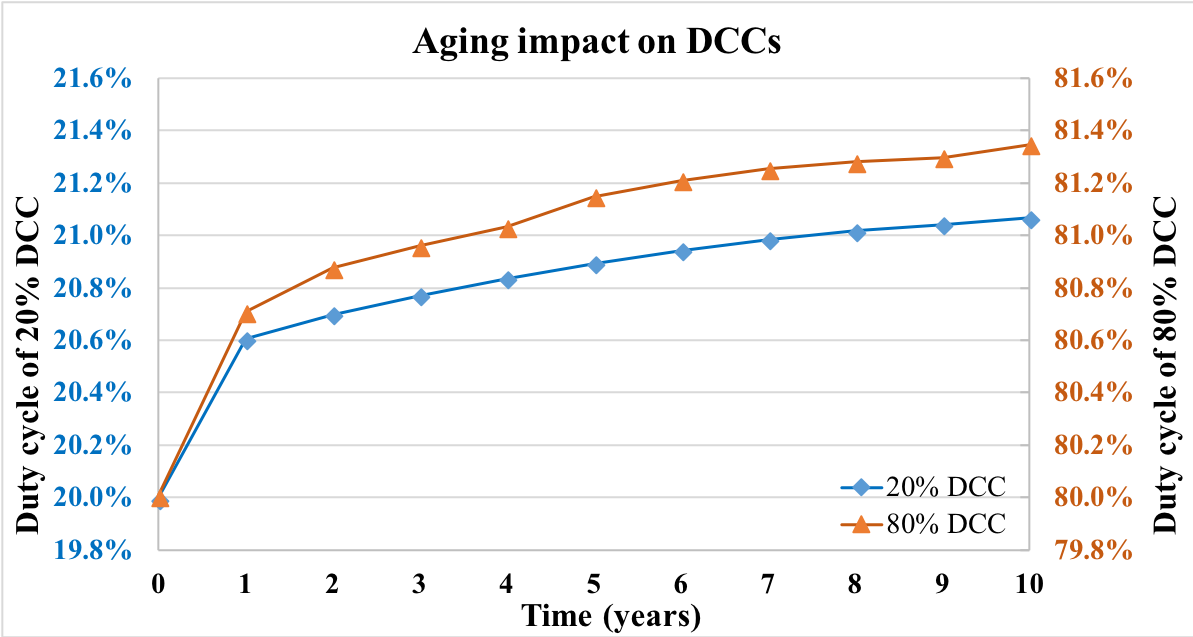
\includegraphics[width=0.9\columnwidth]{Aging_impacted_on_DCC.png} %IEEE
     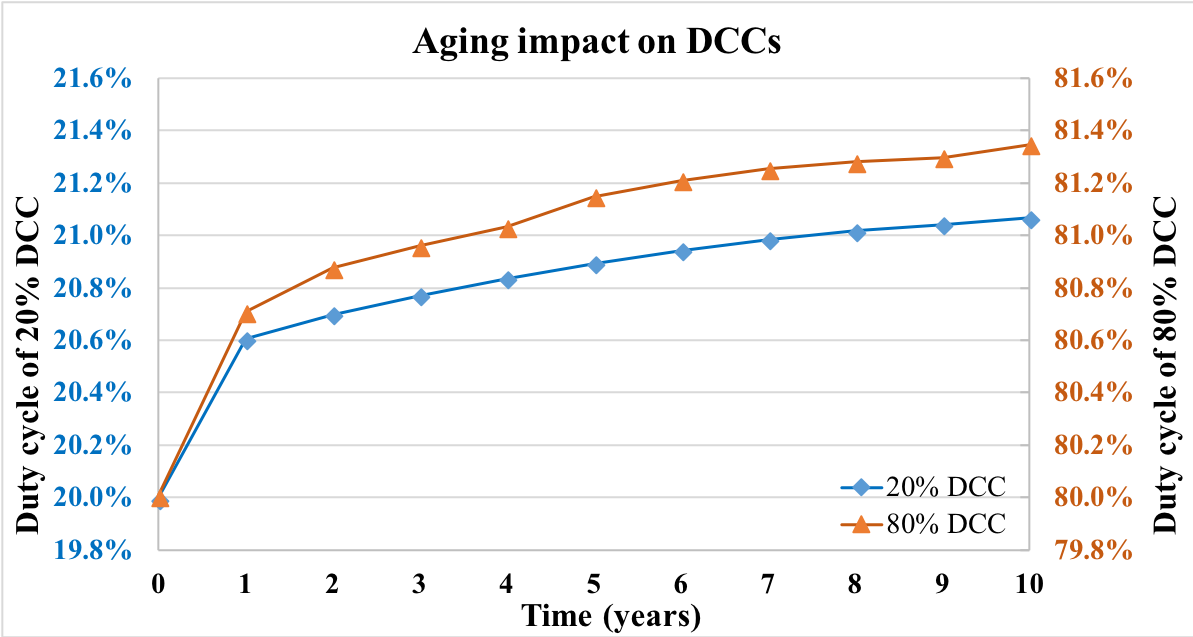
\includegraphics[width=0.6\columnwidth]{Aging_impacted_on_DCC.png} %ACM
    \caption{Aging impact on 20\%/80\% DCC under BTI}
    \label{fig:exp4}
\end{figure}

Figure~\ref{fig:exp4} shows the change in the duty cycle of a 20\%/80\% DCC over 10-year aging. The y axis on the left represents the duty cycle of a 20\% DCC, and the one on the right represents the duty cycle of an 80\% DCC. As it can be seen, the growth in both cases are marginal: $20\% \to 21.07\%$ for a 20\% DCC and $80\% \to 81.35\%$ for an 80\% DCC, which in turn should not affect the benefit of our proposed framework significantly.


\subsection{Discussion: Depth Boundary for DCC Deployment}
\begin{figure}
    \centering
    %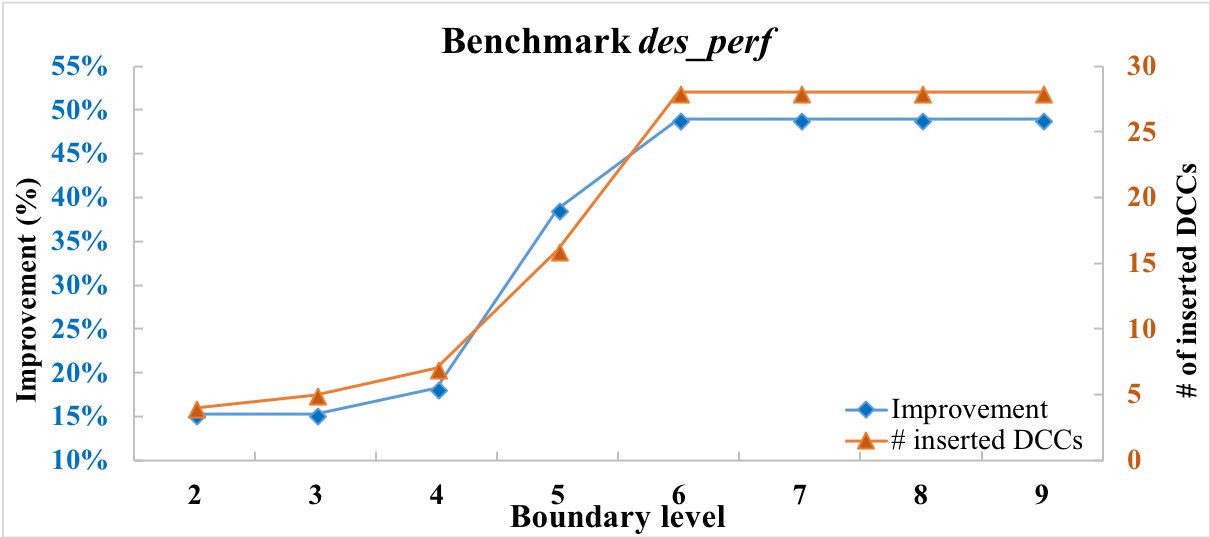
\includegraphics[width=0.9\columnwidth]{Boundary_level_vs_improvement.png} %IEEE
    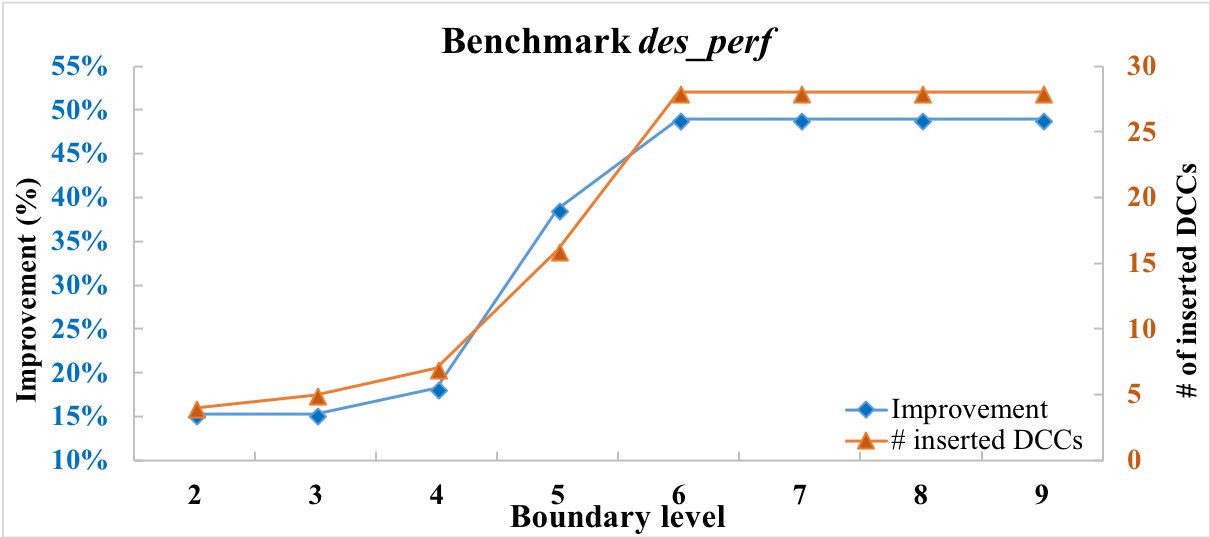
\includegraphics[width=0.6\columnwidth]{Boundary_level_vs_improvement.png} %ACM
    \caption{Improvement/Cost versus clock tree level considered}
    \label{fig:boundary}
\end{figure}

As mentioned in Section~\ref{sec:framework}, inserting DCCs deep in the clock tree is less effective. For benchmark \textit{des\_perf}, we considered the deployment of DCCs at the upper half of the clock tree (i.e., level 1 to 5) and achieved 38.66\% improvement in terms of aging tolerance. As demonstrated in Figure~\ref{fig:boundary}, if we expand the boundary of DCC deployment from level 1 in the clock tree to level 10 progressively, we can gain a considerable improvement from level 1 to 6; however, from 7 to 10, the improvement become stagnant, but more DCCs are required.
\section{CONCLUSION}
\label{sec:conclude}
In this paper, we propose a novel framework, successfully taking advantage of aging-induced clock skews by inserting limited count of DCCs into the clock tree, to enhance circuit aging tolerance. We transform the problem to a Boolean satisfiability formulation which is then solved by using MiniSat. Experiments demonstrate that our framework gains an average of 24.95\% aging tolerance via inserting at most 16 DCCs. Furthermore, we include the mechanism of $V_{th}$ assignment in the framework, to further improve circuit aging tolerance, by assigning small fraction of clock buffers to high $V_{th}$. The problem of selecting buffers to be assigned to high $V_{th}$ is also formulated as a Boolean satisfiability problem, solved by MiniSat. Experiments shows that the framework, which both considers DCC deployment and $V_{th}^h$ assignment for clock buffers, can result in an average of 37.61\% aging tolerance, via inserting at most 35 DCCs and assigning 3.01\% of buffers to high-$V_{th}$.

%------------------- DATE 2018 ------------------------------------------
%In this paper, we propose a novel framework, successfully taking advantage of aging-induced clock skews by inserting limited number of DCCs into the clock tree, to enhance circuit aging tolerance. We transform the problem to a Boolean satisfiability formulation which is then solved by using MiniSat. Experiments demonstrate that our framework gains an average of 25.05\% aging tolerance via inserting at most 15 DCCs and is experimentally verified to be runtime-efficient.

%Process variations (PVs) may shift the delay of each gate, leading to inaccuracy of our optimization results. As indicated in~\cite{wang2010impact}, the transistor with a higher (lower) fresh $V_{th}$ ages at a lower (higher) rate. That is, the variation in $V_{th}$ can be gradually compensated in the aging process. It is demonstrated in~\cite{wang2010impact} that a PV-induced delay shift of 6.2\% can be reduced to 1.6\% after 10-year aging. Even though it is not significant compared to the improvement achieved by our work, we plan to consider the impact of PVs in the future so as to make the proposed idea more robust.



\bibliographystyle{ACM-Reference-Format}
\bibliography{maui}


% that's all folks
\end{document}


